%==========================================================
% Proyecto Final: Localización de una Fuente Sísmica
% Cálculo Multivariable — Universidad Cooperativa de Colombia
% Versión actualizada con análisis del Hessiano, error perfilado
% y referencias académicas extendidas.
%==========================================================

\documentclass[12pt, a4paper]{article}

% --- Idioma y codificación ---
\usepackage[spanish]{babel}
\usepackage[utf8]{inputenc}
\usepackage[T1]{fontenc}

% --- Matemáticas ---
\usepackage{amsmath, amssymb, amsthm}

% --- Figuras y tablas ---
\usepackage{graphicx}
\usepackage{float}
\usepackage{booktabs}
\usepackage{caption}
\usepackage{subcaption}
\usepackage{array}
\usepackage{multirow}

% --- Hipervínculos ---
\usepackage{hyperref}
\hypersetup{
    colorlinks=true,
    linkcolor=blue!60!black,
    citecolor=blue!60!black,
    urlcolor=blue!60!black
}

% --- Márgenes ---
\usepackage{geometry}
\geometry{top=2.5cm, bottom=2.5cm, left=3cm, right=2.5cm}

% --- Interlineado ---
\usepackage{setspace}
\onehalfspacing

% --- Encabezado y pie de página ---
\usepackage{fancyhdr}
\setlength{\headheight}{14pt}
\pagestyle{fancy}
\fancyhf{}
\rhead{\small Localización de Fuente Sísmica --- Problema Inverso}
\lhead{\small Cálculo Multivariable}
\rfoot{\thepage}
\renewcommand{\headrulewidth}{0.4pt}

% --- Ruta de figuras ---
\graphicspath{{../figuras/}}

% --- Utilidades ---
\usepackage{xcolor}
\usepackage{enumitem}
\usepackage{parskip}

%==========================================================
\begin{document}
%==========================================================

%----------------------------------------------------------
% 1. PORTADA
%----------------------------------------------------------
\begin{titlepage}
    \centering
    \vspace*{0.8cm}
    {\Large \textbf{Universidad Cooperativa de Colombia}}\\[0.2cm]
    {\large Facultad de Ingeniería}\\[0.15cm]
    {\large Programa de Ingeniería de Software}\\[2.2cm]

    \rule{\textwidth}{1.5pt}\\[0.5cm]
    {\LARGE \textbf{Localización de una Fuente Sísmica}}\\[0.4cm]
    {\Large \textbf{mediante un Problema Inverso y Datos Simulados}}\\[0.5cm]
    \rule{\textwidth}{1.5pt}\\[2cm]

    {\large \textbf{Integrantes:}}\\[0.4cm]
    \begin{tabular}{l}
        Leider Fabián Chipu Erazo   \\
        Miguel Francisco Ruales     \\
        Juan José Rueda             \\
        Andres Maya                 \\
        Camilo Castro              \\
    \end{tabular}\\[1.8cm]

    {\large \textbf{Asignatura:} Cálculo Multivariable}\\[0.3cm]
    {\large \textbf{Docente:} M.Sc. Alejandro Molina}\\[1.8cm]

    {\large Pasto, Nariño, Colombia}\\[0.2cm]
    
    \vfill
\end{titlepage}

%----------------------------------------------------------
% RESUMEN
%----------------------------------------------------------
\begin{abstract}
\noindent
Se aborda el problema de localización de una fuente sísmica formulado
como un problema inverso no lineal de cuatro parámetros
$\mathbf{m} = (x_0, y_0, z_0, A_0)$. A partir del modelo de atenuación
$A_0\,e^{-R}/R$ para ondas de cuerpo, se simularon datos en ocho
estaciones con ruido gaussiano heteroscedástico moderado
($\alpha = 0.05$). La estimación de los parámetros se abordó mediante
tres métodos complementarios: \emph{(i)} exploración exhaustiva por
grilla tridimensional de $100^3$ puntos con $A_0$ fijo, \emph{(ii)}
\emph{fuerza bruta perfilada}, que estima $\widehat{A}_0(x,y,z)$
analíticamente en cada celda mediante minimización parcial respecto
a $A_0$, y \emph{(iii)} el método iterativo de Levenberg--Marquardt
con backtracking. Los tres enfoques convergen a soluciones consistentes:
errores posicionales de $0.084$, $0.096$ y $0.075$~km, respectivamente.
El análisis espectral del jacobiano en la solución reveló un número
de condición $\kappa = 1.36\times 10^{5}$ y una incertidumbre formal
$\sigma_{z_0} = 0.60$~km, $17$ veces mayor que la incertidumbre
horizontal $\sigma_{x_0}\!\approx\!\sigma_{y_0}\!\approx\!0.035$~km.
La dirección peor resuelta del espacio de parámetros está dominada
en un $90\%$ por $z_0$ con acoplamiento opuesto a $A_0$, constituyendo
evidencia cuantitativa directa del \emph{trade-off} profundidad--amplitud
clásico de la sismología pasiva con redes superficiales.
\end{abstract}

\newpage
\tableofcontents
\listoffigures
\listoftables
\newpage

%----------------------------------------------------------
% 2. INTRODUCCIÓN
%----------------------------------------------------------
\section{Introducción}

\subsection{Contexto del problema sísmico}

La sismología es la disciplina científica que estudia los terremotos
y la propagación de ondas elásticas a través de la Tierra
\cite{shearer2019introduction, stein2003introduction}. Cuando ocurre
un evento sísmico, se generan distintos tipos de ondas que se propagan
desde el \textit{foco} o \textit{hipocentro} —el punto interior donde
se libera la energía— hasta la superficie, donde las registran redes
de estaciones sismográficas. La amplitud de la señal que recibe cada
estación depende de la distancia a la fuente: cuanto mayor es la
distancia, menor es la amplitud, debido a la expansión geométrica
del frente de onda y a la absorción anelástica del medio
\cite{aki1980attenuation, boore2003prediction}.

\subsection{Motivación y relevancia}

Determinar con precisión la ubicación $(x_0, y_0, z_0)$ de una fuente
sísmica es fundamental tanto para la gestión del riesgo sísmico como
para la comprensión de la dinámica interior de la Tierra
\cite{husen2010earthquake}. Este problema es un ejemplo paradigmático
de \textbf{problema inverso}: dados unos datos observados (amplitudes
en estaciones), se buscan los parámetros del modelo que mejor explican
dichos datos \cite{aster2019parameter, tarantola2005inverse}. A
diferencia de un \textit{problema directo} —donde los parámetros son
conocidos y se calculan las observaciones—, el problema inverso
requiere minimizar una función de error que mide la discrepancia
entre lo observado y lo predicho.

Históricamente, la localización sísmica se aborda desde el trabajo
pionero de Geiger \cite{geiger1912probability}, quien formuló el
problema como un sistema linealizado iterativo. Las técnicas modernas
incluyen métodos probabilísticos \cite{lomax2000probabilistic},
diferencias dobles \cite{waldhauser2000double} y enfoques no lineales
robustos \cite{thurber1985nonlinear}.

Desde la perspectiva del \textbf{cálculo multivariable}, este problema
involucra de manera natural varias herramientas centrales del curso:

\begin{itemize}[leftmargin=*, itemsep=2pt]
    \item Construcción y análisis de una función escalar
    $E:\mathbb{R}^4 \to \mathbb{R}_{\geq 0}$ de múltiples variables.
    \item Cálculo del \emph{gradiente} y la \emph{matriz Hessiana} en
    el mínimo.
    \item Aproximación lineal de primer orden mediante el desarrollo
    de Taylor y la matriz \emph{jacobiana}.
    \item Optimización con y sin restricciones, mediante búsqueda
    exhaustiva (fuerza bruta) y métodos iterativos basados en
    derivadas \cite{nocedal2006numerical}.
    \item Estudio de la sensibilidad y estabilidad mediante autovalores
    y autovectores de matrices simétricas \cite{golub2013matrix}.
\end{itemize}

Estas herramientas tienen aplicaciones directas en ingeniería,
geofísica, aprendizaje automático y ciencias aplicadas.

\subsection{Objetivos}

\textbf{Objetivo general:} Analizar y estimar la localización de una
fuente sísmica mediante la minimización de una función de error
dependiente de múltiples variables, utilizando herramientas de cálculo
multivariable, simulación numérica y visualización.

\textbf{Objetivos específicos:}
\begin{enumerate}[label=\roman*.]
    \item Construir una función de error $E(x, y, z)$ que cuantifique
    la diferencia entre los datos observados y los predichos por el
    modelo de atenuación sísmica.
    \item Explorar el comportamiento de la función de error en el
    espacio tridimensional mediante cortes bidimensionales $z = k$
    (mapas de calor).
    \item Identificar, para cada plano $z = k$, los puntos $(x, y)$
    que minimizan la función de error.
    \item Construir la función reducida
    $E_{\min}(z) = \min_{x,y} E(x,y,z)$ y determinar el valor de $z$
    que produce el menor error global.
    \item Analizar la dependencia de la solución $(x^*(z), y^*(z))$
    y evaluar la estabilidad y sensibilidad del resultado.
    \item Implementar y comparar un método iterativo de mínimos
    cuadrados basado en el jacobiano del sistema.
    \item Cuantificar la incertidumbre de los parámetros estimados
    mediante el análisis espectral del Hessiano del problema.
    \item Interpretar los resultados en términos físicos, relacionando
    la estructura de la función de error con la calidad de la
    estimación.
\end{enumerate}

%----------------------------------------------------------
% 3. MARCO TEÓRICO
%----------------------------------------------------------
\section{Marco Teórico}

\subsection{Modelo de atenuación de amplitudes sísmicas}

Para ondas de cuerpo que se propagan en un medio homogéneo e isótropo,
la amplitud disminuye con la distancia a la fuente por dos razones
principales: la \textit{expansión geométrica} del frente de onda
(proporcional a $1/R$, consecuencia de la conservación de energía
sobre superficies esféricas) y la \textit{absorción anelástica} del
medio (proporcional a $e^{-R}$, derivada del modelo de Aki para
atenuación intrínseca \cite{aki1980attenuation}). El modelo
simplificado adoptado en este proyecto combina ambos efectos:

\begin{equation}
    A_{z_i} = A_0 \, \frac{e^{-R_i}}{R_i} + \epsilon_i
    \label{eq:modelo}
\end{equation}

donde $A_0$ es la amplitud sísmica en el origen (en el foco), $R_i$ es
la distancia euclidiana entre la fuente y la estación $i$, y
$\epsilon_i$ es un término de ruido aleatorio. La distancia se calcula
como:

\begin{equation}
    R_i = \sqrt{(x_i - x_0)^2 + (y_i - y_0)^2 + (z_i - z_0)^2}
    \label{eq:distancia}
\end{equation}

siendo $(x_i, y_i, z_i)$ la posición conocida de la estación $i$ y
$(x_0, y_0, z_0)$ la posición desconocida de la fuente. La amplitud
predicha sin ruido es:

\begin{equation}
    A'_{z_i} = A_0 \, \frac{e^{-R_i}}{R_i}
    \label{eq:predicha}
\end{equation}

La función $f(R) = e^{-R}/R$ es estrictamente decreciente para $R > 0$,
garantizando que estaciones más lejanas registren amplitudes menores.

\subsection{Modelo de ruido gaussiano}

El término $\epsilon_i$ modela las imperfecciones instrumentales y del
medio. Se representa mediante una distribución normal centrada en
$\mu = 0$:

\begin{equation}
    f(\epsilon) = \frac{1}{\sqrt{2\pi\sigma_i^2}}
    \exp\!\left(-\frac{(\epsilon - \mu)^2}{2\sigma_i^2}\right)
    \label{eq:ruido}
\end{equation}

La desviación estándar $\sigma_i$ es proporcional a la amplitud limpia
en cada estación:

\begin{equation}
    \sigma_i = \alpha \cdot A_0 \, \frac{e^{-R_i}}{R_i}
    \label{eq:sigma}
\end{equation}

con $\alpha = 0.05$ (ruido moderado del $5\%$). Esta elección produce
un ruido \textit{heteroscedástico}: la relación señal-ruido se mantiene
constante en todas las estaciones. La media $\mu = 0$ asegura que no
haya sesgo sistemático en las mediciones, condición esencial para que
los estimadores de mínimos cuadrados sean insesgados
\cite{menke2018geophysical}.

\subsection{Formulación del problema inverso}

Se define el vector de parámetros del modelo:

\begin{equation}
    \mathbf{m} = [x_0,\; y_0,\; z_0,\; A_0]^T \in \mathbb{R}^4
    \label{eq:parametros}
\end{equation}

y el vector de amplitudes observadas en $M = 8$ estaciones:

\begin{equation}
    \mathbf{A}_z = [A_{z_1},\; A_{z_2},\; \ldots,\; A_{z_M}]^T \in \mathbb{R}^M
    \label{eq:observados}
\end{equation}

El problema inverso consiste en encontrar $\mathbf{m}^*$ tal que las
amplitudes predichas se aproximen óptimamente a las observadas.

\subsection{Función de error}

Bajo el supuesto de ruido gaussiano independiente, el estimador de
máxima verosimilitud coincide con el estimador de mínimos cuadrados
\cite{aster2019parameter, menke2018geophysical}. Adoptamos por tanto
el criterio:

\begin{equation}
    E(\mathbf{m}) = \sum_{i=1}^{M} \left(A_{z_i} - A'_{z_i}(\mathbf{m})\right)^2
    = \sum_{i=1}^{M} \left(A_{z_i} - A_0\,\frac{e^{-R_i}}{R_i}\right)^2
    \label{eq:error}
\end{equation}

El problema de localización se reduce a:

\begin{equation}
    \mathbf{m}^* = \arg\min_{\mathbf{m} \in \mathbb{R}^4}\; E(\mathbf{m})
    \label{eq:minimo}
\end{equation}

Esta función no tiene forma cerrada para su mínimo, ya que la
dependencia de $R_i$ respecto a $(x_0, y_0, z_0)$ es no lineal, lo
que impide resolverla analíticamente igualando el gradiente a cero.

\subsubsection*{Función de error perfilada en \texorpdfstring{$A_0$}{A0}}

Una observación importante es que $A_0$ aparece como factor lineal
en el modelo (Ec.~\ref{eq:predicha}). Por lo tanto, para
$(x,y,z)$ \emph{fijos}, el mínimo de $E$ con respecto a $A_0$ se
obtiene en forma cerrada. Derivando $\partial E/\partial A_0 = 0$:

\begin{equation}
    -2 \sum_{i=1}^{M} \left( A_{z_i} - A_0\,u_i\right) u_i = 0,
    \qquad u_i \equiv \frac{e^{-R_i}}{R_i}
\end{equation}

de donde:

\begin{equation}
    \widehat{A}_0(x, y, z) = \frac{\sum_{i=1}^M A_{z_i}\,u_i}{\sum_{i=1}^M u_i^2}
    \label{eq:A0_perfilado}
\end{equation}

Sustituyendo de vuelta en \eqref{eq:error} se obtiene la \emph{función
de error perfilada}:

\begin{equation}
    \widetilde{E}(x, y, z) =
    \sum_{i=1}^{M} \left( A_{z_i} - \widehat{A}_0(x,y,z)\,u_i \right)^2
    \label{eq:error_perfilado}
\end{equation}

Esta forma reduce el problema 4D original a uno 3D equivalente, sin
necesidad de fijar $A_0$ a priori. Es una técnica estándar en problemas
inversos, conocida como \emph{variable projection}
\cite{nocedal2006numerical} y permite una comparación justa entre la
búsqueda por grilla y el método iterativo.

\subsection{Linealización y método iterativo de mínimos cuadrados}

Dado que el modelo es no lineal en $(x_0, y_0, z_0)$, se linealiza
alrededor de una aproximación inicial $\mathbf{m}_0$ mediante el
desarrollo de Taylor de primer orden:

\begin{equation}
    A_{z_i}(\mathbf{m}) \approx A_{z_i}(\mathbf{m}_0)
    + \sum_{j=1}^{4} \left.\frac{\partial A_{z_i}}{\partial m_j}
    \right|_{\mathbf{m}_0} \!\!\Delta m_j
    \label{eq:taylor}
\end{equation}

Definiendo $\Delta\mathbf{m} = \mathbf{m} - \mathbf{m}_0$ y
$\Delta\mathbf{A}_z = \mathbf{A}_z - \mathbf{A}_z(\mathbf{m}_0)$,
el sistema se escribe matricialmente como:

\begin{equation}
    \Delta\mathbf{A}_z \approx \mathbf{G}\,\Delta\mathbf{m}
    \label{eq:sistema_matricial}
\end{equation}

donde $\mathbf{G}$ es la \textbf{matriz jacobiana} de dimensión
$M \times 4$. Las derivadas parciales analíticas se obtienen aplicando
la regla de la cadena. Sea $g(R) = e^{-R}/R$; entonces
$dg/dR = -e^{-R}(R+1)/R^2$, y como
$\partial R_i/\partial x_0 = -(x_i-x_0)/R_i$, se tiene:

\begin{align}
    \frac{\partial A_{z_i}}{\partial x_0} &=
    A_0\,e^{-R_i}\,\frac{(x_i - x_0)}{R_i^2}
    \left(\frac{1}{R_i} + 1\right) \label{eq:dAdx}\\[4pt]
    \frac{\partial A_{z_i}}{\partial y_0} &=
    A_0\,e^{-R_i}\,\frac{(y_i - y_0)}{R_i^2}
    \left(\frac{1}{R_i} + 1\right) \label{eq:dAdy}\\[4pt]
    \frac{\partial A_{z_i}}{\partial z_0} &=
    A_0\,e^{-R_i}\,\frac{(z_i - z_0)}{R_i^2}
    \left(\frac{1}{R_i} + 1\right) \label{eq:dAdz}\\[4pt]
    \frac{\partial A_{z_i}}{\partial A_0} &=
    \frac{e^{-R_i}}{R_i} \label{eq:dAdA0}
\end{align}

\noindent\textbf{Derivación paso a paso de la Ecuación~\eqref{eq:dAdx}:}

\begin{align*}
    \frac{\partial A_{z_i}}{\partial x_0}
    &= A_0 \cdot \frac{d}{dR}\!\left(\frac{e^{-R}}{R}\right)
       \cdot \frac{\partial R_i}{\partial x_0} \\[4pt]
    &= A_0 \cdot \left(\frac{-e^{-R_i}\cdot R_i - e^{-R_i}}{R_i^2}\right)
       \cdot \left(\frac{-(x_i - x_0)}{R_i}\right) \\[4pt]
    &= A_0 \cdot \left(\frac{-e^{-R_i}(R_i + 1)}{R_i^2}\right)
       \cdot \left(\frac{-(x_i - x_0)}{R_i}\right) \\[4pt]
    &= A_0\,e^{-R_i}\,\frac{(x_i - x_0)(R_i + 1)}{R_i^3}
     = A_0\,e^{-R_i}\,\frac{(x_i - x_0)}{R_i^2}
       \left(\frac{1}{R_i} + 1\right)
\end{align*}

Las derivadas respecto a $y_0$ y $z_0$ son análogas por simetría.
La Ecuación~\eqref{eq:dAdA0} se obtiene directamente ya que $A_0$
aparece como factor lineal en el modelo.

\subsubsection*{Esquema iterativo de Levenberg--Marquardt}

La solución en cada iteración se obtiene mediante mínimos cuadrados
con regularización adaptativa de tipo Levenberg--Marquardt
\cite{levenberg1944method, marquardt1963algorithm}:

\begin{equation}
    \Delta\mathbf{m} = \left(\mathbf{G}^T\mathbf{G} +
    \lambda_k\mathbf{I}\right)^{-1} \mathbf{G}^T \,\Delta\mathbf{A}_z
    \label{eq:LM}
\end{equation}

con $\lambda_k$ ajustado dinámicamente en cada iteración (ver
Sección~\ref{sec:metodo_iterativo}), y la actualización del modelo:

\begin{equation}
    \mathbf{m}_{k+1} = \mathbf{m}_k + \Delta\mathbf{m}
    \label{eq:actualizacion}
\end{equation}

La regularización $\lambda_k\mathbf{I}$ es esencial cuando
$\mathbf{G}^T\mathbf{G}$ es mal condicionada \cite{tikhonov1963regularization};
en el límite $\lambda_k\to 0$ se recupera Gauss-Newton puro
(convergencia cuadrática cerca del mínimo), y en el límite
$\lambda_k\to\infty$ se aproxima al descenso por gradiente (paso
corto pero garantizado de descenso). La estrategia de
\emph{backtracking} de Levenberg--Marquardt combina ambas, ajustando
$\lambda$ en función del éxito o fracaso del paso. El proceso se
repite hasta $\|\Delta\mathbf{m}\| < \varepsilon$ o $k = k_{\max}$.

\subsection{Análisis de incertidumbre vía la matriz de información}
\label{sec:teoria_covarianza}

En la solución $\hat{\mathbf{m}}$, la matriz Hessiana de la función
de error vale aproximadamente $H = 2\,\mathbf{G}^T\mathbf{G}$, ya que
los términos de segundo orden son despreciables cuando los residuales
son pequeños \cite{nocedal2006numerical, bjorck1996numerical}. Bajo
el supuesto de ruido gaussiano homoscedástico (o tras una adecuada
ponderación en el caso heteroscedástico), la \emph{matriz de
covarianza} de los parámetros estimados es:

\begin{equation}
    \widehat{\mathbf{C}}
    = \hat{\sigma}^2 \,(\mathbf{G}^T\mathbf{G})^{-1},
    \qquad
    \hat{\sigma}^2 = \frac{E^*}{M - p}
    \label{eq:covarianza}
\end{equation}

donde $E^*$ es el residual cuadrático en el mínimo, $M=8$ es el número
de estaciones y $p=4$ el número de parámetros. Los elementos diagonales
$C_{jj}$ definen las \emph{barras de error} $\sigma_{m_j} = \sqrt{C_{jj}}$
de cada parámetro \cite{aster2019parameter, menke2018geophysical}.

La descomposición espectral
$\mathbf{G}^T\mathbf{G} = \mathbf{V}\boldsymbol{\Lambda}\mathbf{V}^T$
con autovalores $\lambda_1 \ge \cdots \ge \lambda_p$ identifica las
direcciones del espacio de parámetros que están mejor y peor
resueltas por los datos \cite{backus1968resolving}. El \emph{número
de condición}:

\begin{equation}
    \kappa = \frac{\lambda_{\max}}{\lambda_{\min}}
    \label{eq:condicion}
\end{equation}

cuantifica el mal condicionamiento del problema: valores $\kappa \gg 1$
indican que pequeñas perturbaciones en los datos producen grandes
cambios en la solución \cite{golub2013matrix}. Aplicaremos este análisis
en la Sección~\ref{sec:analisis_hessiano}.

%----------------------------------------------------------
% 4. METODOLOGÍA
%----------------------------------------------------------
\section{Metodología}

La implementación se realizó en \texttt{Python}~3.11 utilizando las
librerías \texttt{NumPy} \cite{harris2020array}, \texttt{SciPy}
\cite{virtanen2020scipy} y \texttt{Matplotlib} \cite{hunter2007matplotlib}.
El código completo está organizado modularmente y se encuentra
disponible en el repositorio público referenciado en el
Apéndice~\ref{apx:repo}.

\subsection{Configuración de estaciones y parámetros simulados}

Se definieron $M = 8$ estaciones sísmicas distribuidas para cubrir
distintos cuadrantes y profundidades del área de estudio. La
distribución azimutal completa es deliberada: garantiza que la matriz
$\mathbf{G}^T\mathbf{G}$ no sea degenerada y que las direcciones
$x_0$ y $y_0$ estén bien restringidas por los datos.

\begin{table}[H]
    \centering
    \caption{Coordenadas de las estaciones sísmicas (km).}
    \label{tab:estaciones}
    \begin{tabular}{clrrr}
        \toprule
        \textbf{Estación} & \textbf{Descripción} &
        $x_i$ & $y_i$ & $z_i$ \\
        \midrule
        S1 & Noroeste, superficie       & $-5.0$ & $ 4.0$ & $ 0.0$ \\
        S2 & Norte, superficie          & $ 0.0$ & $ 5.0$ & $ 0.0$ \\
        S3 & Noreste, superficie        & $ 5.0$ & $ 3.0$ & $ 0.0$ \\
        S4 & Oeste, profundidad leve    & $-4.0$ & $ 0.0$ & $-0.5$ \\
        S5 & Este, profundidad leve     & $ 4.0$ & $ 0.0$ & $-0.5$ \\
        S6 & Suroeste                   & $-3.0$ & $-4.0$ & $-0.3$ \\
        S7 & Sur                        & $ 2.0$ & $-5.0$ & $-0.2$ \\
        S8 & Sureste, superficie        & $ 6.0$ & $-3.0$ & $ 0.0$ \\
        \bottomrule
    \end{tabular}
\end{table}

Es importante notar que todas las estaciones están en el rango
$z_i \in [-0.5, 0]$~km, es decir, son esencialmente \emph{superficiales}.
Esta característica geométrica tendrá consecuencias directas sobre la
resolución vertical del problema, como se analizará en la
Sección~\ref{sec:sensibilidad_z}.

Los parámetros reales del sismo simulado se fijaron como:

\begin{equation}
    \mathbf{m}_{\text{real}} =
    [x_0,\; y_0,\; z_0,\; A_0]^T =
    [-1.0,\; 0.5,\; -1.2,\; 2.0]^T
    \label{eq:m_real}
\end{equation}

La posición fue elegida descentrada respecto al arreglo de estaciones,
con profundidad real de $1.2$~km, evitando simetrías artificiales que
facilitarían la inversión.

\subsection{Simulación de datos con ruido}

Para cada estación $i$ se sigue el procedimiento:

\begin{enumerate}[itemsep=2pt]
    \item Cálculo de la distancia $R_i$ (Ec.~\ref{eq:distancia}).
    \item Amplitud limpia $A'_{z_i} = A_0\,e^{-R_i}/R_i$
    (Ec.~\ref{eq:predicha}).
    \item Desviación estándar del ruido:
    $\sigma_i = \alpha \cdot A'_{z_i}$, con $\alpha = 0.05$.
    \item Muestra de ruido $\epsilon_i \sim \mathcal{N}(0,\,\sigma_i^2)$.
    \item Amplitud observada: $A_{z_i} = A'_{z_i} + \epsilon_i$.
\end{enumerate}

Se utilizó la semilla aleatoria \texttt{seed} $= 42$ a través del
generador moderno \texttt{numpy.random.default\_rng}, garantizando
reproducibilidad exacta de los resultados.

\subsection{Construcción de la función de error}

Se implementaron \emph{dos versiones} complementarias de la función
de error, lo que permite contrastar las metodologías y discutir el
trade-off profundidad--amplitud:

\paragraph{Versión 1 — $A_0$ fijo a su valor real.}
Fijando $A_0 = 2.0$, la función se escribe:
\begin{equation}
    E(x, y, z) = \sum_{i=1}^{8}
    \left(A_{z_i} - 2.0\,\frac{e^{-R_i(x,y,z)}}{R_i(x,y,z)}\right)^2
    \label{eq:error_explicito}
\end{equation}
Esta versión es útil para visualizar la función como un campo
escalar en $\mathbb{R}^3$ (mapas de calor) y para generar la
animación de la Fase~5.

\paragraph{Versión 2 — Función de error perfilada.}
Usando la Ec.~\eqref{eq:A0_perfilado}, $\widehat{A}_0(x,y,z)$ se
estima analíticamente en cada celda. La función perfilada
$\widetilde{E}(x,y,z)$ (Ec.~\ref{eq:error_perfilado}) se evalúa
sobre la misma grilla y proporciona la versión 3D del problema 4D
original, permitiendo una comparación honesta con el método
iterativo.

Ambas versiones son continuas y diferenciables para todo $(x,y,z)$
distinto de las posiciones de las estaciones, no negativas, y su
mínimo teórico (sin ruido) sería cero en $(x_0, y_0, z_0)$.

\subsection{Exploración por grilla tridimensional}

Se evalúan ambas funciones de error en una grilla regular de
$100\times100\times100 = 10^6$ puntos en el dominio
$x \in [-8, 8]$~km, $y \in [-8, 8]$~km, $z \in [-3, 0]$~km. La
implementación usa vectorización con NumPy \cite{harris2020array}:
para cada corte $z_k$ se construye un arreglo de $10\,000$ candidatos
y se evalúan simultáneamente las distancias a las 8 estaciones
mediante \emph{broadcasting} matricial. La función reducida es:

\begin{equation}
    E_{\min}(z) = \min_{x,\,y}\; E(x, y, z)
    \label{eq:emin}
\end{equation}

\subsubsection*{Análisis de curvatura local}
\label{sec:curvatura_local}

Para cuantificar la sensibilidad del problema respecto a $z$, ajustamos
una parábola a $E_{\min}(z)$ en una ventana de $15$ puntos centrada en
$z^*$:

\begin{equation}
    E_{\min}(z) \approx E^* + \tfrac{1}{2}\,c\,(z - z^*)^2
    \label{eq:parabola}
\end{equation}

La curvatura $c = d^2 E_{\min}/dz^2\big|_{z^*}$ es una medida directa
de cuán "agudo" es el pozo: valores grandes implican alta sensibilidad
en profundidad. Definimos el \emph{ancho local} del pozo como el
intervalo donde la aproximación parabólica duplica el mínimo:

\begin{equation}
    \Delta z_{\text{local}} = 2\sqrt{\frac{2\, E^*}{c}}
    \label{eq:ancho_local}
\end{equation}

Esta caracterización mediante la segunda derivada constituye un
ejemplo directo del uso del cálculo multivariable para analizar la
sensibilidad de un problema de inversión.

\subsection{Método iterativo: Levenberg--Marquardt con backtracking}
\label{sec:metodo_iterativo}

Se implementa el esquema de Levenberg--Marquardt
(Ec.~\ref{eq:LM}--\ref{eq:actualizacion}) con $k_{\max} = 200$ y
tolerancia $\varepsilon = 10^{-8}$. A diferencia de un Gauss--Newton
puro, la versión implementada incluye:

\begin{itemize}[leftmargin=*, itemsep=2pt]
    \item \textbf{Backtracking adaptativo:} en cada iteración se prueba
    el paso propuesto; si reduce el error, se acepta y $\lambda$ se
    divide por $10$; si lo aumenta, se rechaza y $\lambda$ se multiplica
    por $10$, repitiendo hasta encontrar un paso útil. Esto garantiza
    descenso monótono y robustez ante mal condicionamiento.
    \item \textbf{Filtro físico:} se rechaza cualquier paso que
    produzca $A_0 \le 0$, ya que la amplitud debe ser estrictamente
    positiva por la física del problema. Sin este filtro, el método
    diverge cuando un paso de Gauss-Newton crudo lleva $A_0$ a valores
    negativos.
    \item \textbf{Detección de piso de ruido:} si el algoritmo no puede
    reducir más el error pero las correcciones recientes son pequeñas
    ($\|\Delta\mathbf{m}\| < 10^{-4}$), se considera convergencia al
    \emph{piso de ruido} (no es posible mejorar más debido al ruido
    presente en los datos).
\end{itemize}

Se prueban cuatro puntos de partida para evaluar la robustez del
método:

\begin{table}[H]
    \centering
    \caption{Puntos de partida para el método iterativo.}
    \label{tab:inicios}
    \begin{tabular}{lrrrr}
        \toprule
        \textbf{Escenario} &
        $x_0^{(0)}$ & $y_0^{(0)}$ & $z_0^{(0)}$ & $A_0^{(0)}$ \\
        \midrule
        Cerca del mínimo       & $ 0.0$ & $ 0.0$ & $-1.0$ & $1.5$ \\
        Lejos NE               & $ 4.0$ & $ 4.0$ & $-0.5$ & $1.0$ \\
        Lejos SO               & $-5.0$ & $-5.0$ & $-2.0$ & $3.0$ \\
        Muy cerca del mínimo   & $-0.5$ & $ 0.0$ & $-1.0$ & $2.0$ \\
        \bottomrule
    \end{tabular}
\end{table}

\subsection{Análisis de incertidumbre en la solución}

En la solución estimada $\hat{\mathbf{m}}$ se calcula:
\begin{enumerate}[itemsep=2pt]
    \item El jacobiano $\mathbf{G} \in \mathbb{R}^{8\times 4}$.
    \item La matriz de covarianza $\widehat{\mathbf{C}}$
    (Ec.~\ref{eq:covarianza}).
    \item Las barras de error $\sigma_{m_j} = \sqrt{C_{jj}}$ para
    cada parámetro.
    \item Los autovalores y autovectores de $\mathbf{G}^T\mathbf{G}$,
    para identificar las direcciones bien y mal resueltas.
    \item El número de condición $\kappa$ (Ec.~\ref{eq:condicion}).
\end{enumerate}

%----------------------------------------------------------
% 5. RESULTADOS
%----------------------------------------------------------
\section{Resultados}

\subsection{Datos simulados}

\begin{table}[H]
    \centering
    \caption{Datos sísmicos simulados ($A_0=2.0$, $\alpha=0.05$,
    \texttt{seed}$=42$).}
    \label{tab:datos}
    \begin{tabular}{crrrrr}
        \toprule
        \textbf{Est.} & $R_i$ (km) & $A'_{z_i}$ & $A_{z_i}$ (obs.) &
        $\epsilon_i$ & $\sigma_i$ \\
        \midrule
        S1 & 5.4489 & 0.001579 & 0.001603 & $+0.000024$ & 0.000079 \\
        S2 & 4.7634 & 0.003584 & 0.003398 & $-0.000186$ & 0.000179 \\
        S3 & 6.6098 & 0.000408 & 0.000423 & $+0.000015$ & 0.000020 \\
        S4 & 3.1209 & 0.028272 & 0.029602 & $+0.001330$ & 0.001414 \\
        S5 & 5.0735 & 0.002468 & 0.002227 & $-0.000241$ & 0.000123 \\
        S6 & 5.0060 & 0.002676 & 0.002502 & $-0.000174$ & 0.000134 \\
        S7 & 6.3443 & 0.000554 & 0.000557 & $+0.000004$ & 0.000028 \\
        S8 & 7.9177 & 0.000092 & 0.000091 & $-0.000001$ & 0.000005 \\
        \bottomrule
    \end{tabular}
\end{table}

S4 es la más cercana ($R_4 = 3.12$~km) con la amplitud más alta;
S8 la más lejana ($R_8 = 7.92$~km) con amplitud casi nula. Los ruidos
$\epsilon_i$ son en todos los casos menores al $5\%$ de la amplitud
limpia, verificando el nivel establecido. La
Figura~\ref{fig:fase1} muestra la geometría del sistema y la
atenuación de las amplitudes.

\begin{figure}[H]
    \centering
    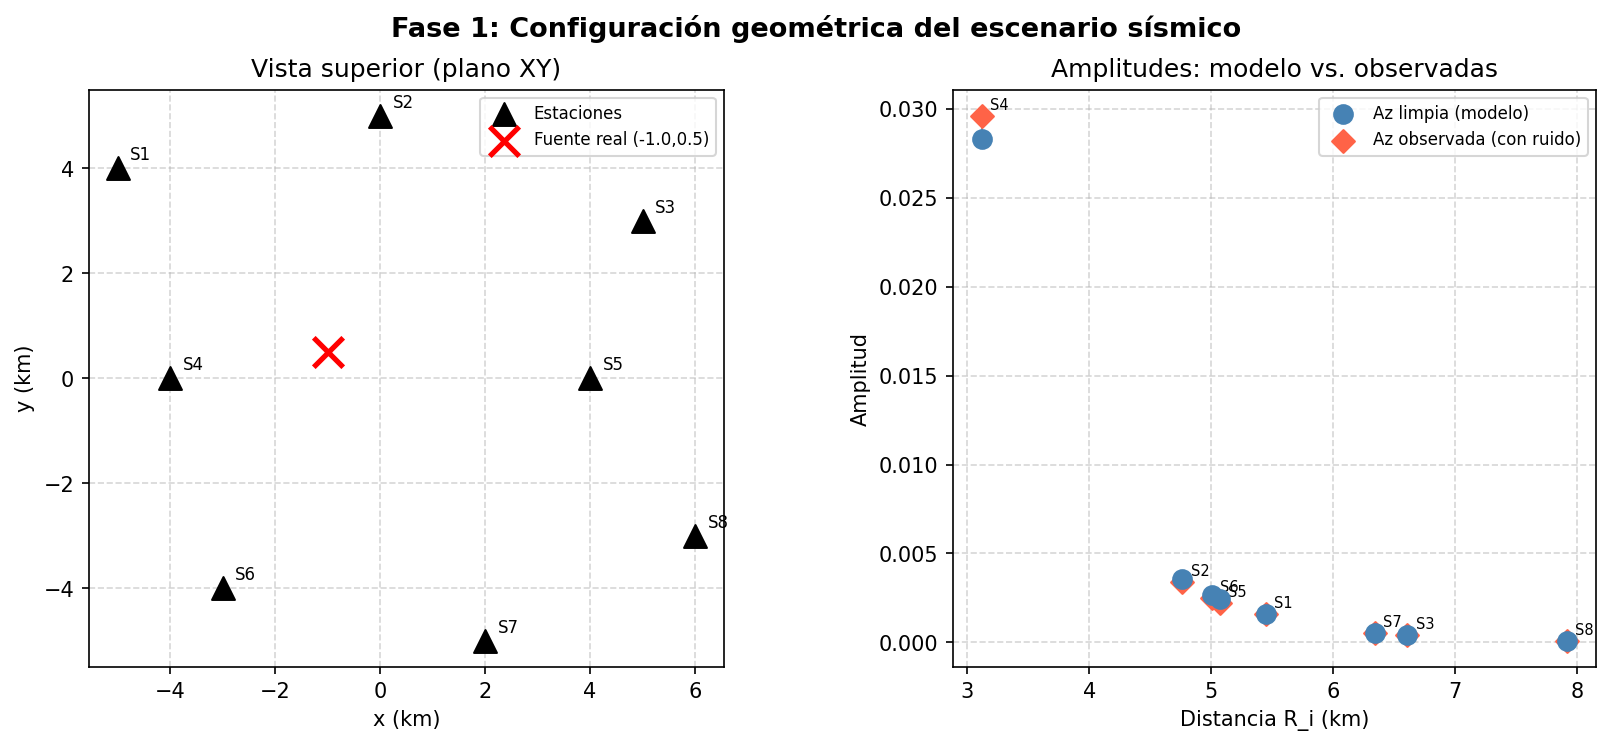
\includegraphics[width=0.97\textwidth]{fase1_verificacion.png}
    \caption{Izquierda: distribución de las 8 estaciones (triángulos)
    y la fuente real (cruz roja) en el plano $XY$. Derecha: amplitudes
    limpias (azul) vs. observadas con ruido (rojo) en función de la
    distancia $R_i$. Las líneas punteadas muestran la magnitud del
    ruido $\epsilon_i$ en cada estación.}
    \label{fig:fase1}
\end{figure}

\subsection{Mapas de calor por cortes \texorpdfstring{$z = k$}{z=k}}

\begin{figure}[H]
    \centering
    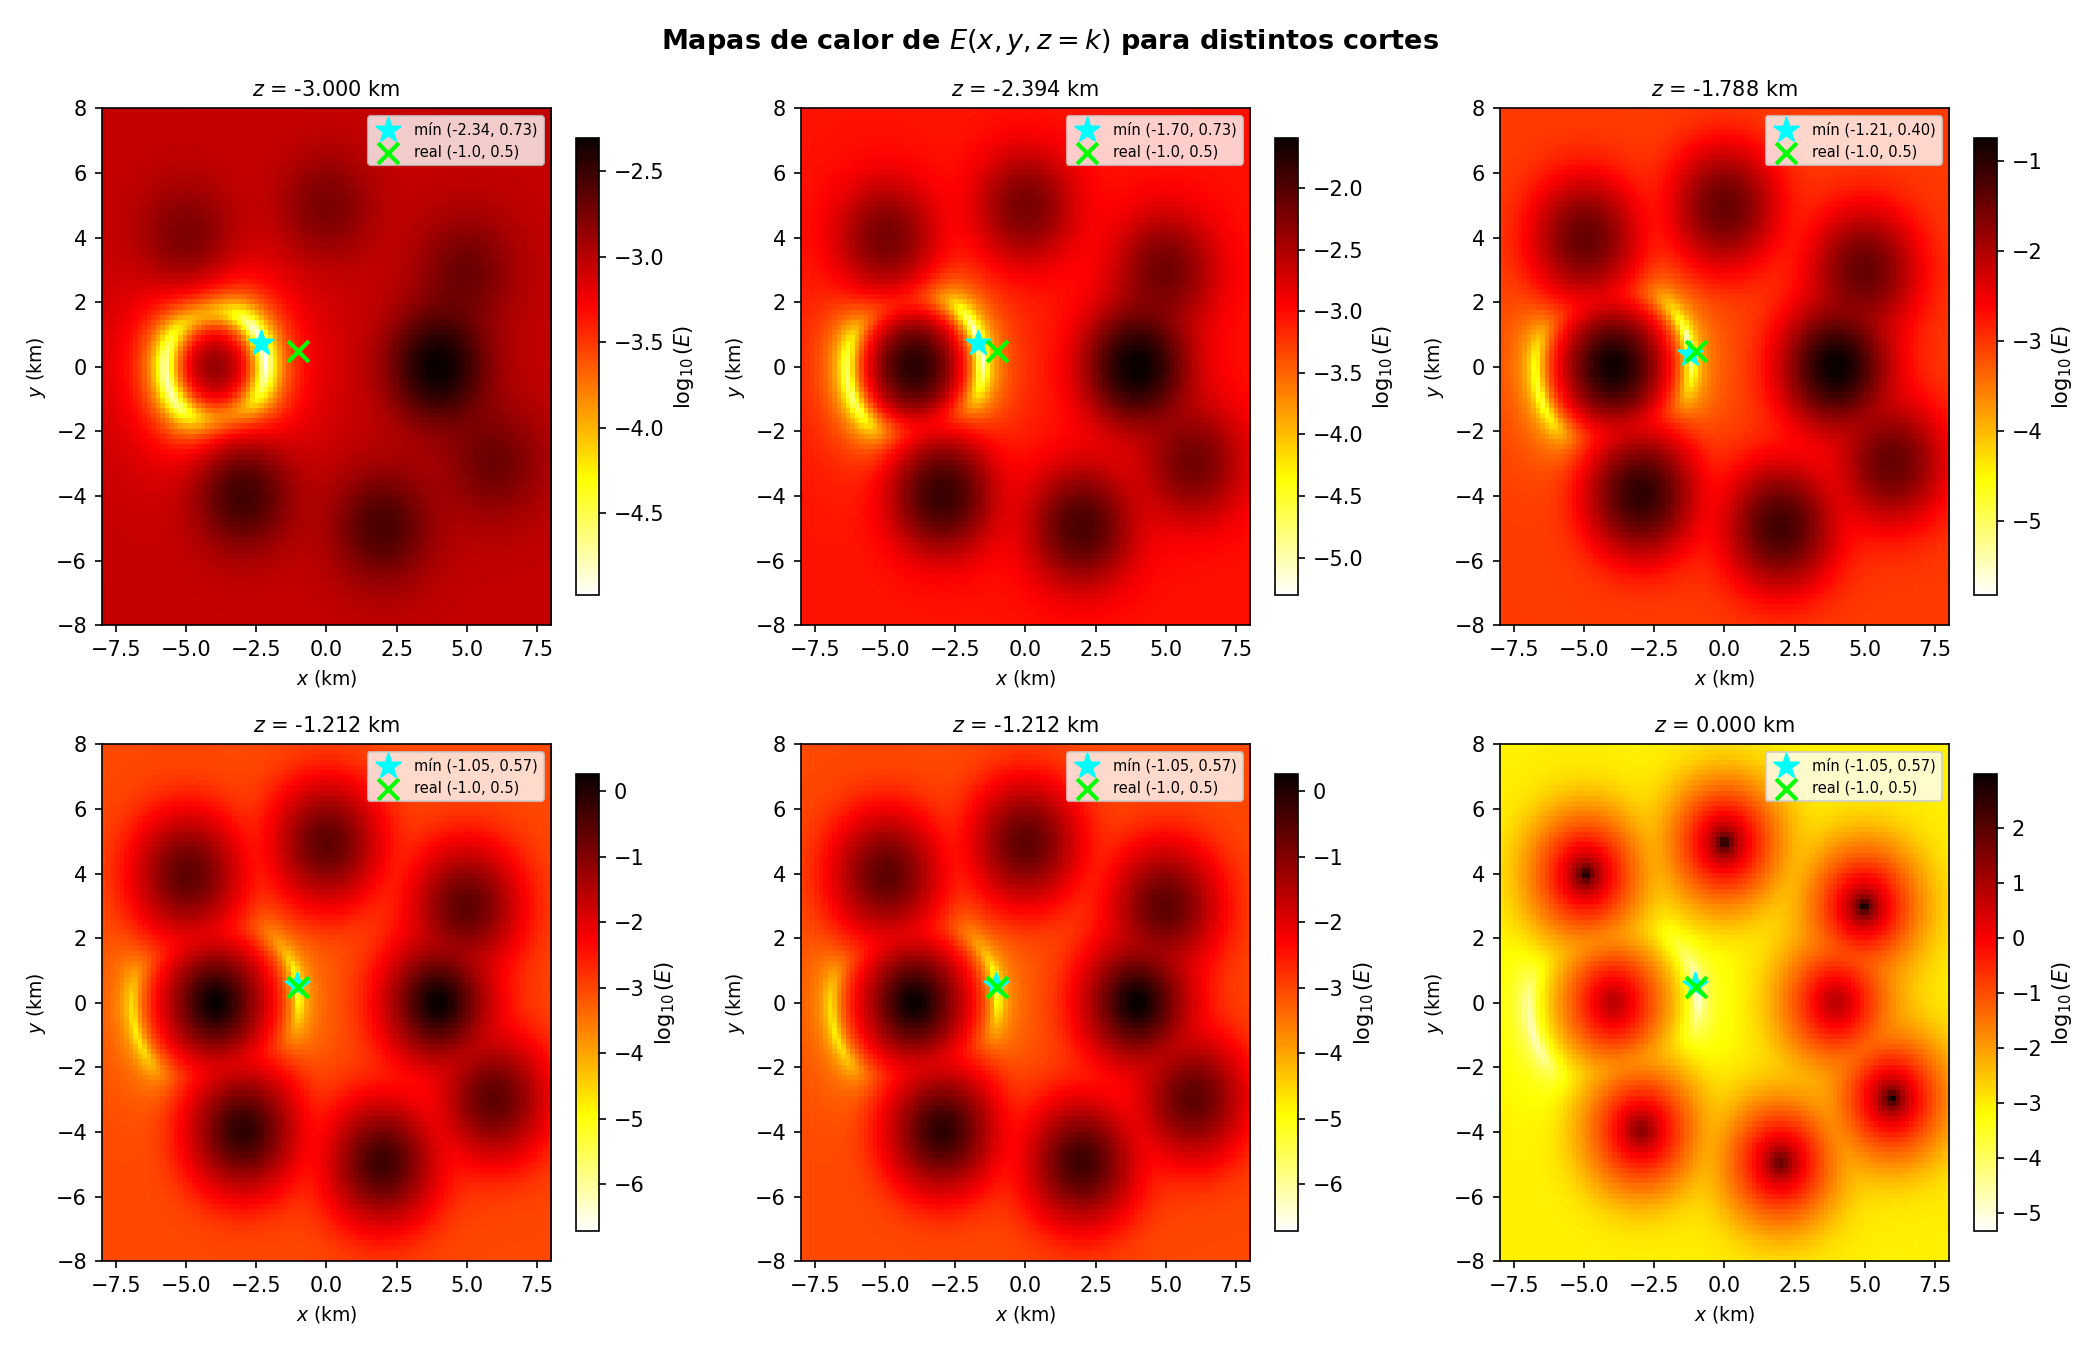
\includegraphics[width=0.97\textwidth]{heatmaps/heatmaps_selected.png}
    \caption{Mapas de calor de $\log_{10}[E(x,y,z=k)]$ para seis
    valores de $z$. Las estrellas cyan indican el mínimo de $E$ en
    cada corte; las cruces verdes la posición real. A medida que $z$
    se acerca a $z^* = -1.212$~km, la mancha oscura (baja energía)
    se concentra y el mínimo se localiza con mayor precisión.}
    \label{fig:heatmaps}
\end{figure}

\begin{figure}[H]
    \centering
    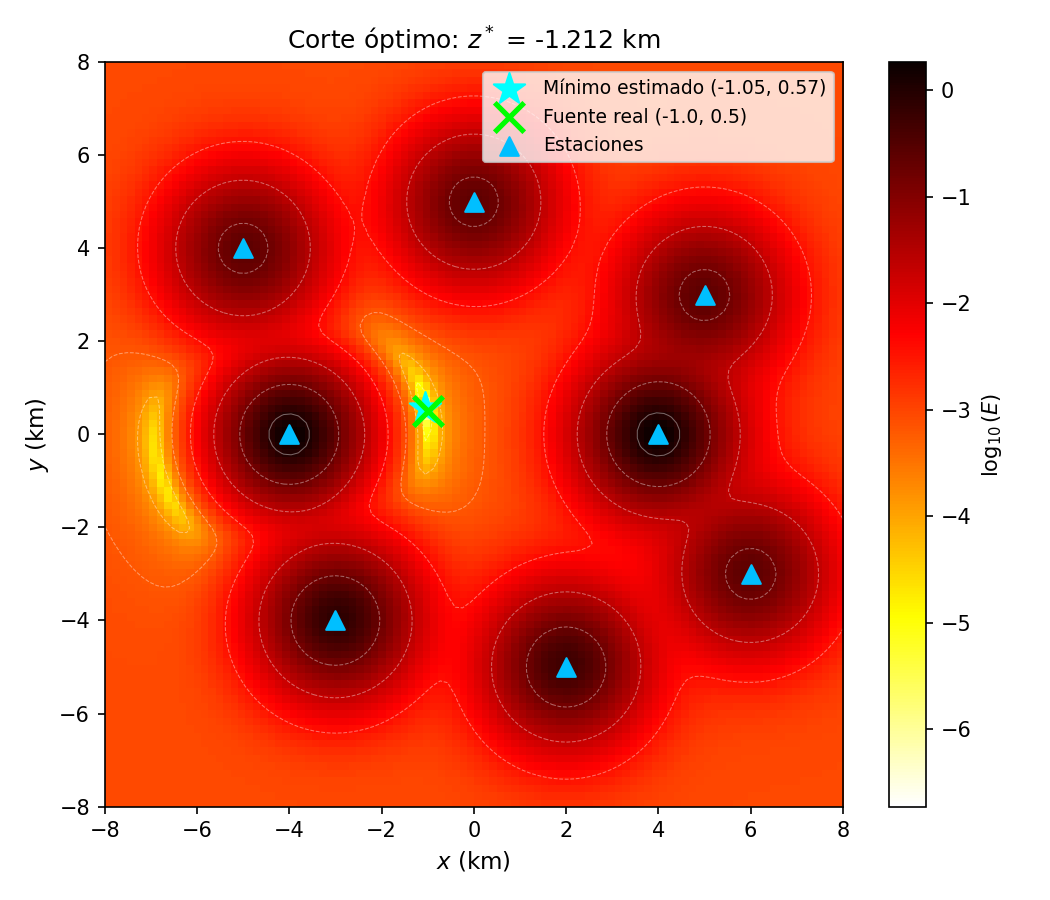
\includegraphics[width=0.78\textwidth]{heatmaps/heatmap_optimal.png}
    \caption{Corte detallado en el plano óptimo $z^* = -1.212$~km,
    con líneas de contorno en blanco para evidenciar la forma
    elipsoidal del mínimo. Triángulos azules: estaciones; estrella
    cyan: mínimo estimado; cruz verde: fuente real.}
    \label{fig:heatmap_opt}
\end{figure}

\subsection{Curva \texorpdfstring{$E_{\min}(z)$}{Emin(z)} y profundidad estimada}

\begin{figure}[H]
    \centering
    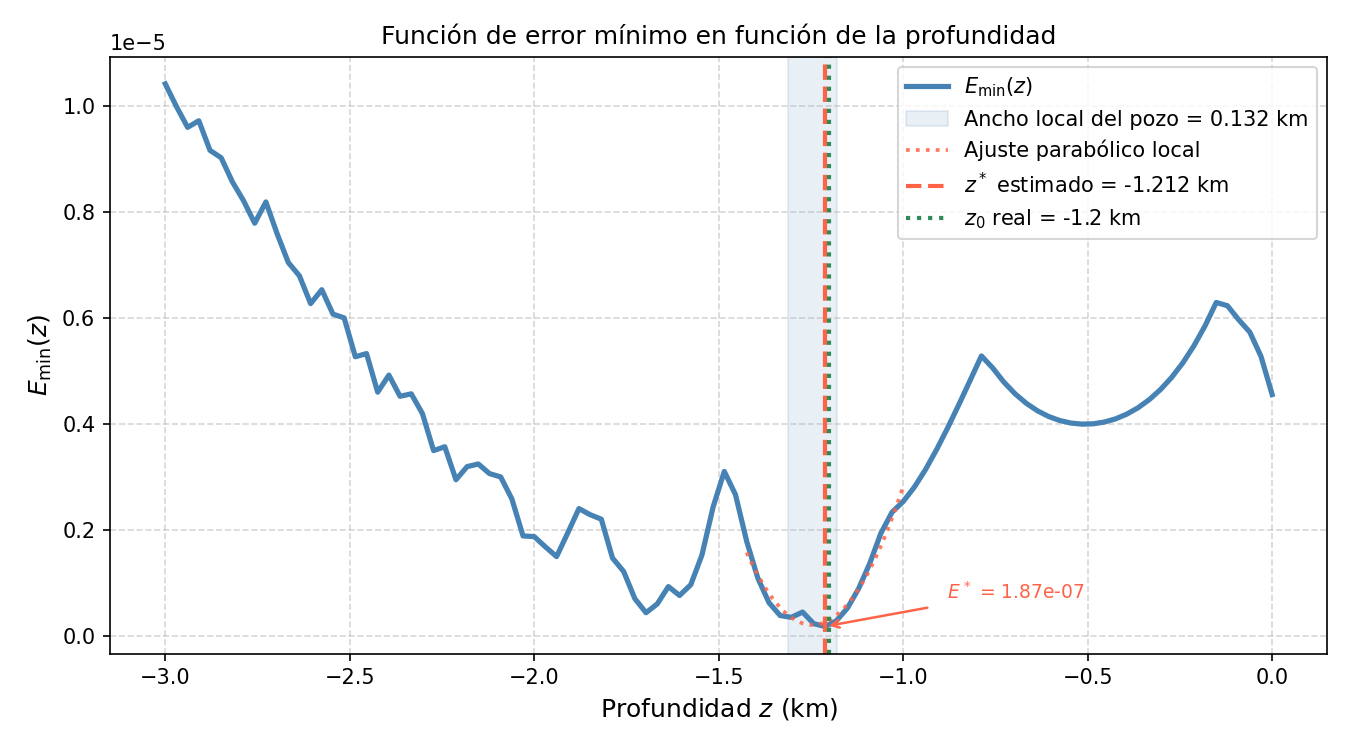
\includegraphics[width=0.88\textwidth]{curva_emin.png}
    \caption{Función reducida $E_{\min}(z)$. La línea roja punteada
    indica $z^* = -1.212$~km (estimado), la línea verde $z_0 = -1.2$~km
    (real). La banda sombreada y la curva punteada roja indican,
    respectivamente, el ancho local del pozo y el ajuste parabólico
    en su vecindad.}
    \label{fig:emin}
\end{figure}

\begin{figure}[H]
    \centering
    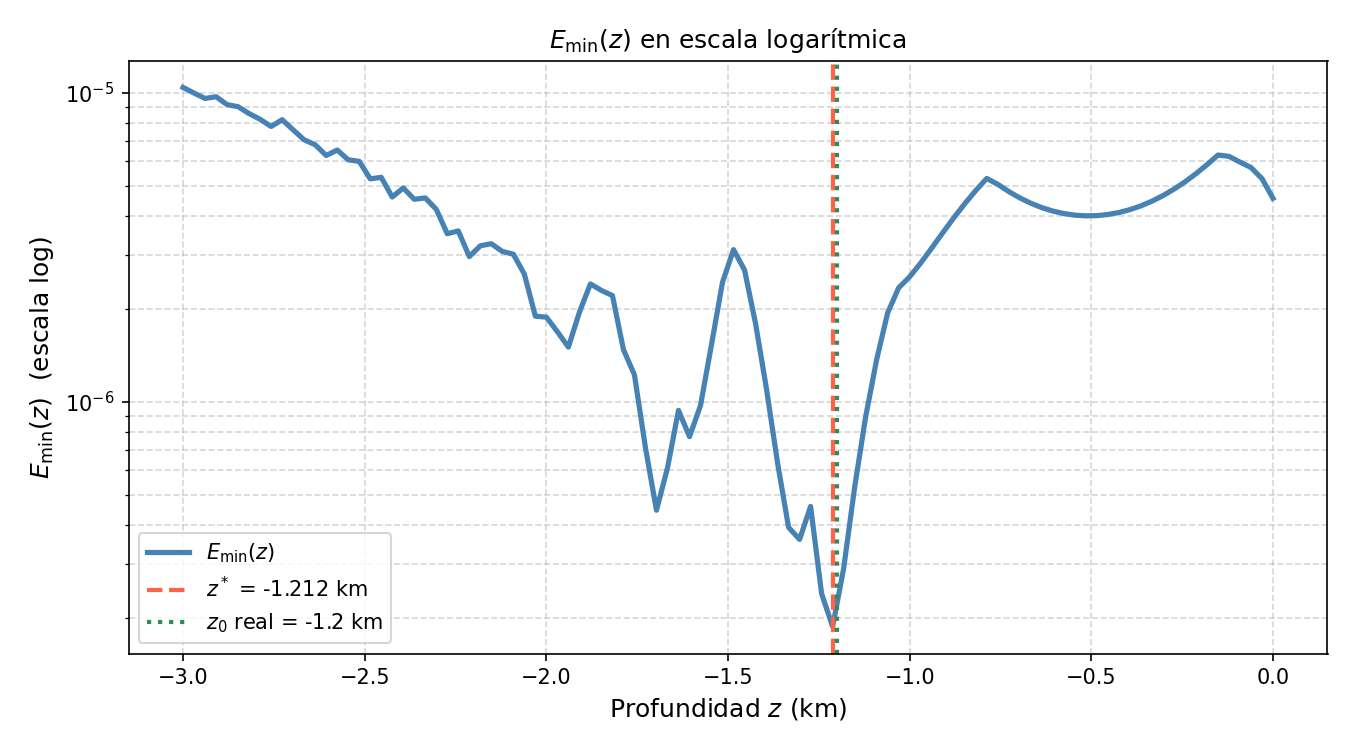
\includegraphics[width=0.88\textwidth]{curva_emin_log.png}
    \caption{$E_{\min}(z)$ en escala logarítmica. Permite apreciar
    el pozo mínimo y la asimetría: el flanco derecho (hacia $z=0$)
    es más abrupto que el izquierdo (hacia $z=-3$~km).}
    \label{fig:emin_log}
\end{figure}

El análisis cuantitativo de la curvatura local en el mínimo
(Sección~\ref{sec:curvatura_local}) arroja:

\begin{itemize}[leftmargin=*, itemsep=2pt]
    \item Profundidad óptima: $z^* = -1.212$~km (error de $0.012$~km
    respecto al valor real).
    \item Mínimo de la función reducida: $E^* = 1.874 \times 10^{-7}$.
    \item Curvatura ajustada: $d^2 E_{\min}/dz^2\big|_{z^*}
    = 8.62 \times 10^{-5}$.
    \item Ancho local del pozo (intervalo donde $\widetilde{E}\le 2E^*$):
    $\Delta z_{\text{local}} = 0.132$~km.
\end{itemize}

Este ancho local es notablemente más pequeño que el ancho de la curva
en regiones lejanas al mínimo, indicando que cerca del óptimo la
función está bien definida pero pierde sensibilidad rápidamente al
alejarse.

\subsection{Trayectoria \texorpdfstring{$(x^*(z),\, y^*(z))$}{(x*(z), y*(z))}}

\begin{figure}[H]
    \centering
    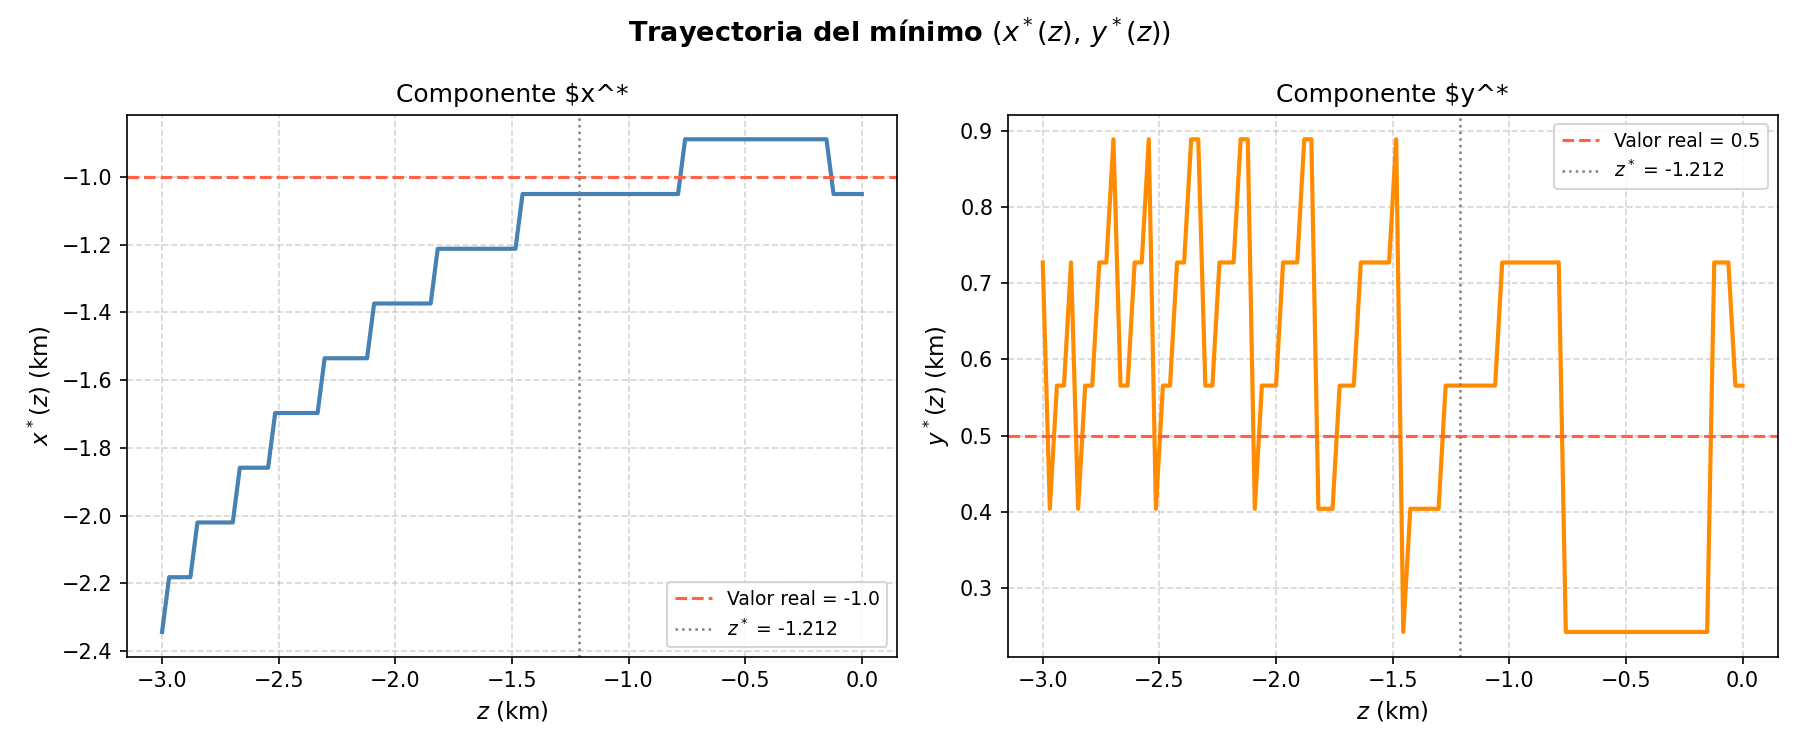
\includegraphics[width=0.95\textwidth]{trayectoria_xy.png}
    \caption{Evolución de $(x^*(z), y^*(z))$ al variar $z$. Las líneas
    rojas punteadas marcan los valores reales $x_0=-1.0$~km y
    $y_0=0.5$~km. La línea gris vertical indica $z^*=-1.212$~km.
    La estructura escalonada para $z$ alejado de $z^*$ es un
    artefacto de la discretización de la grilla y es coherente con
    la baja resolución del mínimo en esa región.}
    \label{fig:trayectoria}
\end{figure}

\subsection{Fuerza bruta perfilada}

La función de error perfilada $\widetilde{E}(x,y,z)$, evaluada en la
misma grilla 3D, permite estimar simultáneamente los cuatro parámetros
sin fijar $A_0$ a priori. El mínimo global da:

\begin{equation*}
    (x^*, y^*, z^*, \widehat{A}_0) = (-1.051,\; 0.566,\; -1.151,\; 1.962)
\end{equation*}

con $E^* = 1.834 \times 10^{-7}$ y error posicional $0.096$~km.

\begin{figure}[H]
    \centering
    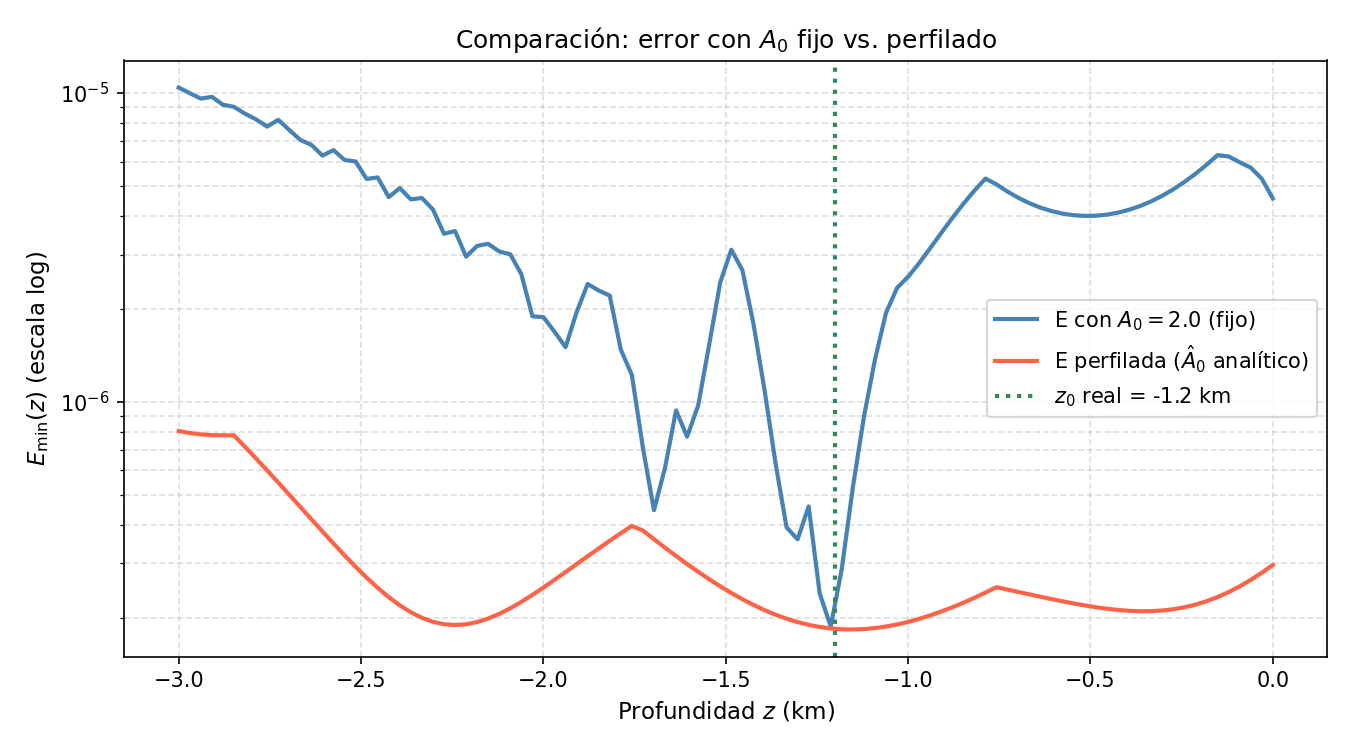
\includegraphics[width=0.95\textwidth]{comparacion_perfilada.png}
    \caption{Comparación entre $E_{\min}(z)$ con $A_0 = 2.0$ fijo
    (azul) y la versión perfilada con $\widehat{A}_0$ analítico
    (rojo). La perfilada está sistemáticamente por debajo, lo que
    es matemáticamente esperable: un parámetro libre adicional solo
    puede reducir (o igualar) el mínimo del residual.}
    \label{fig:comparacion_perfilada}
\end{figure}

\begin{figure}[H]
    \centering
    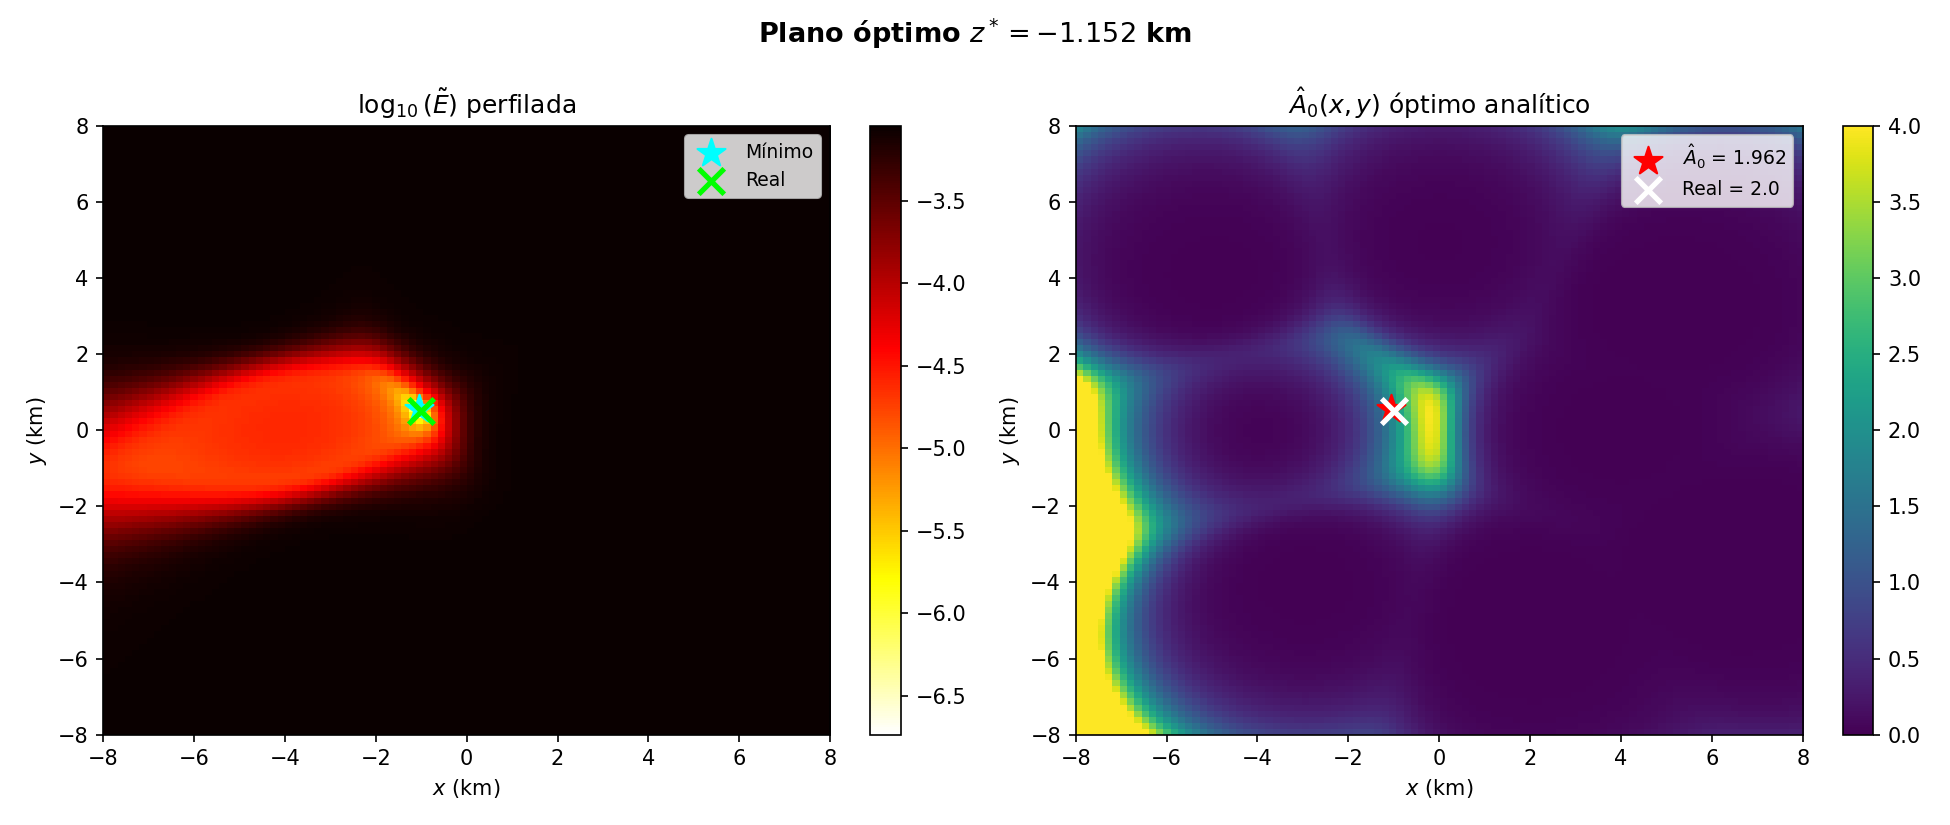
\includegraphics[width=0.95\textwidth]{mapa_A0_perfilado.png}
    \caption{Plano óptimo $z^* = -1.152$~km de la fuerza bruta
    perfilada. Izquierda: error perfilado $\log_{10}\widetilde{E}$.
    Derecha: amplitud estimada $\widehat{A}_0(x,y)$ en el mismo plano.
    En el mínimo del error, $\widehat{A}_0 \approx 1.96$, próximo
    al valor real $A_0 = 2.0$.}
    \label{fig:mapa_A0}
\end{figure}

\subsection{Convergencia del método iterativo}

\begin{figure}[H]
    \centering
    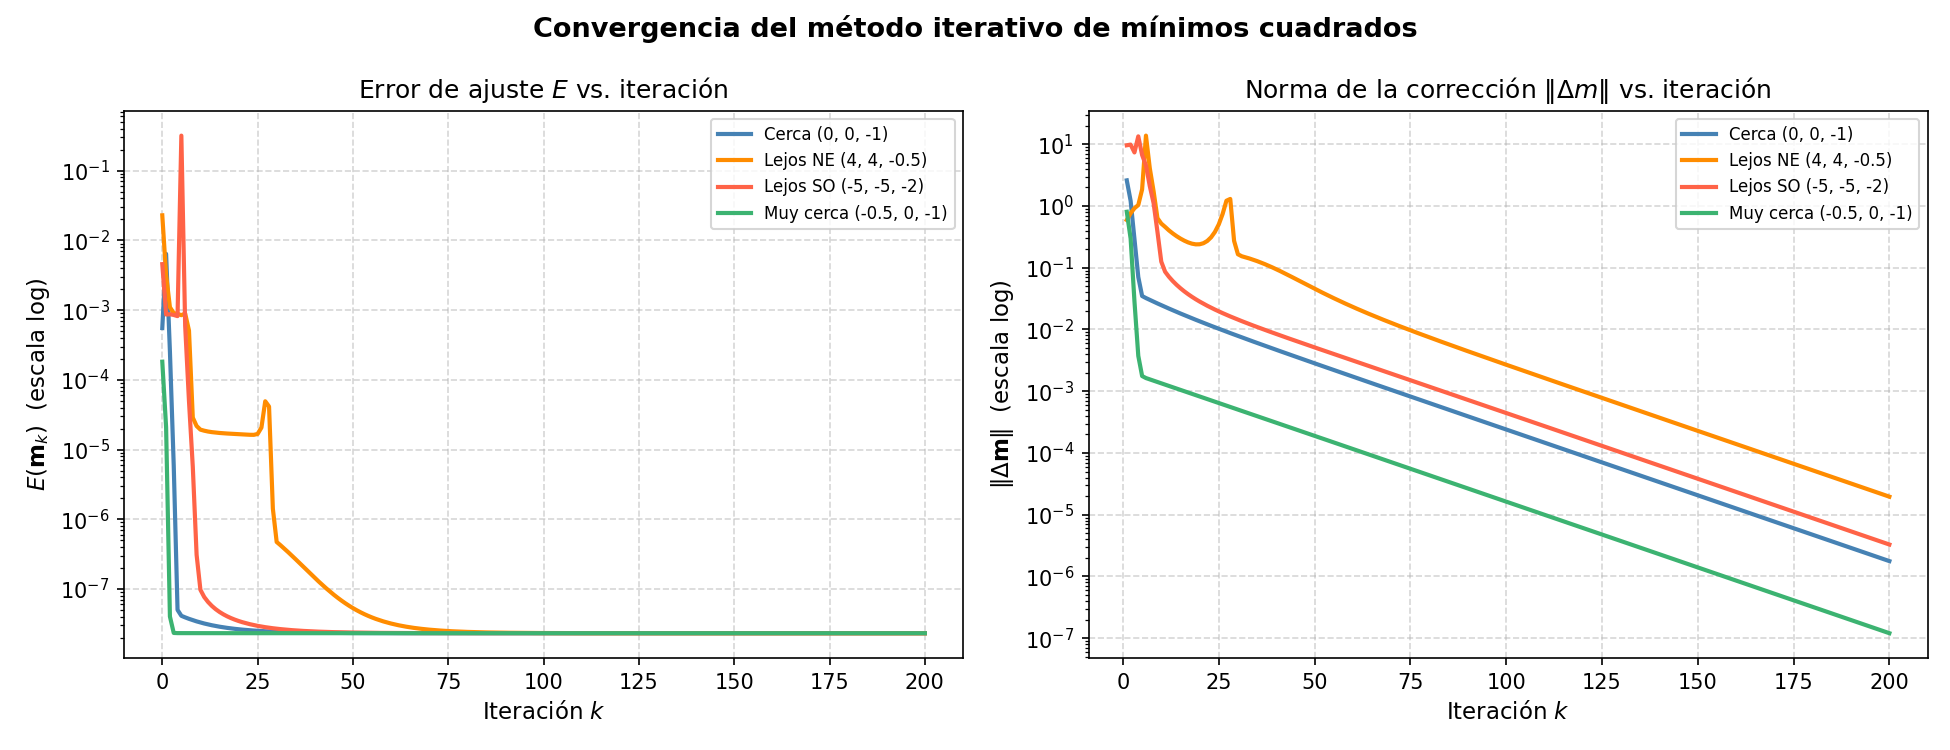
\includegraphics[width=0.95\textwidth]{convergencia.png}
    \caption{Izquierda: evolución de $E(\mathbf{m}_k)$ en escala
    logarítmica para los cuatro puntos de partida. Derecha: norma
    $\|\Delta\mathbf{m}\|$ por iteración. Todos los inicios convergen
    al mismo nivel de error, demostrando robustez del método de
    Levenberg--Marquardt.}
    \label{fig:convergencia}
\end{figure}

\begin{figure}[H]
    \centering
    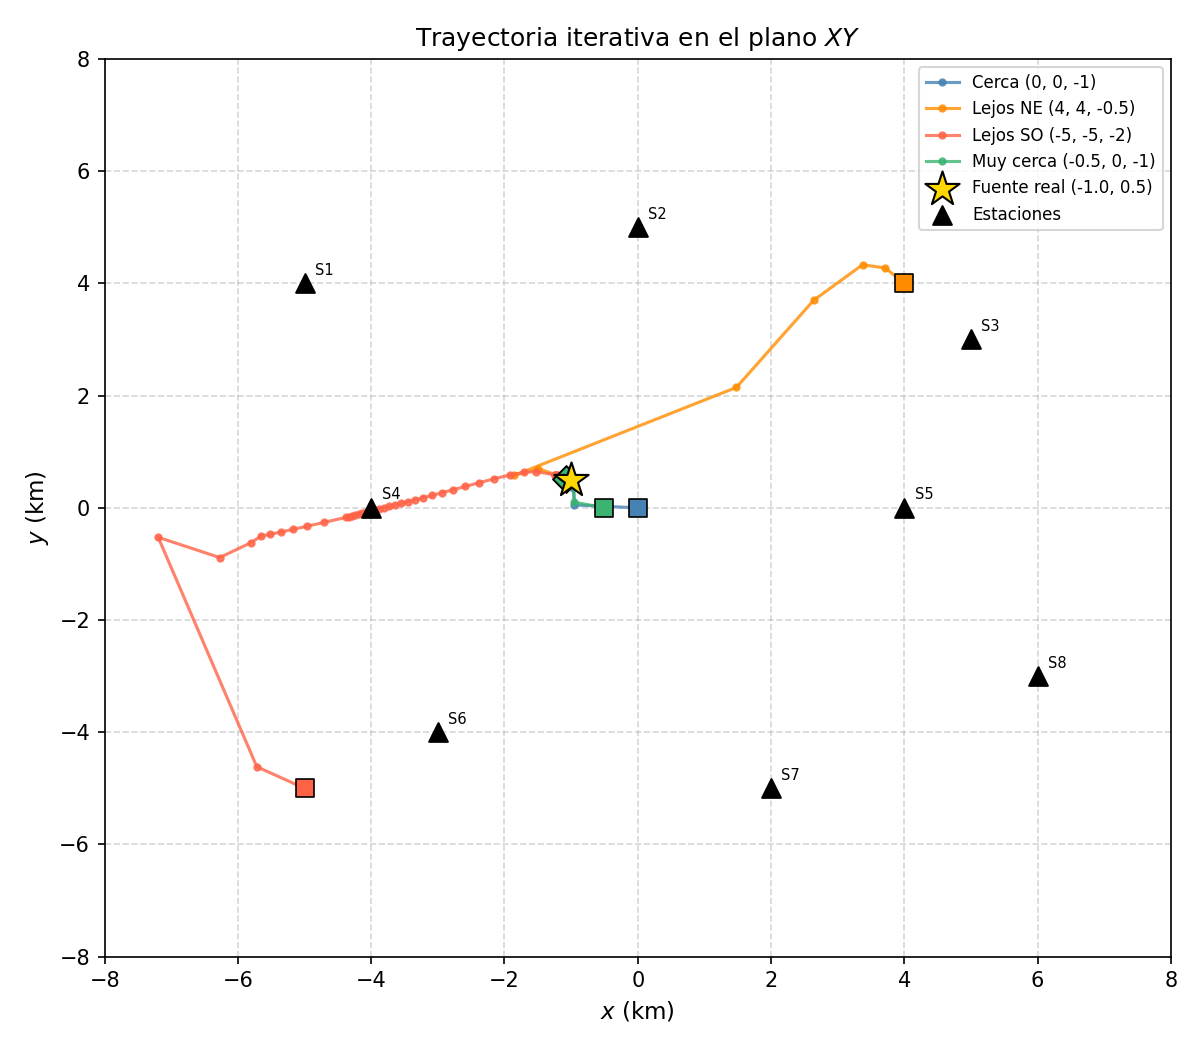
\includegraphics[width=0.78\textwidth]{trayectoria_iterativa.png}
    \caption{Trayectorias iterativas en el plano $XY$. Los cuadrados
    son puntos iniciales; los rombos, puntos finales. La estrella
    dorada es la fuente real. Todos los inicios convergen a la misma
    solución final, validando empíricamente la unicidad del mínimo
    en el dominio explorado.}
    \label{fig:tray_iter}
\end{figure}

\begin{figure}[H]
    \centering
    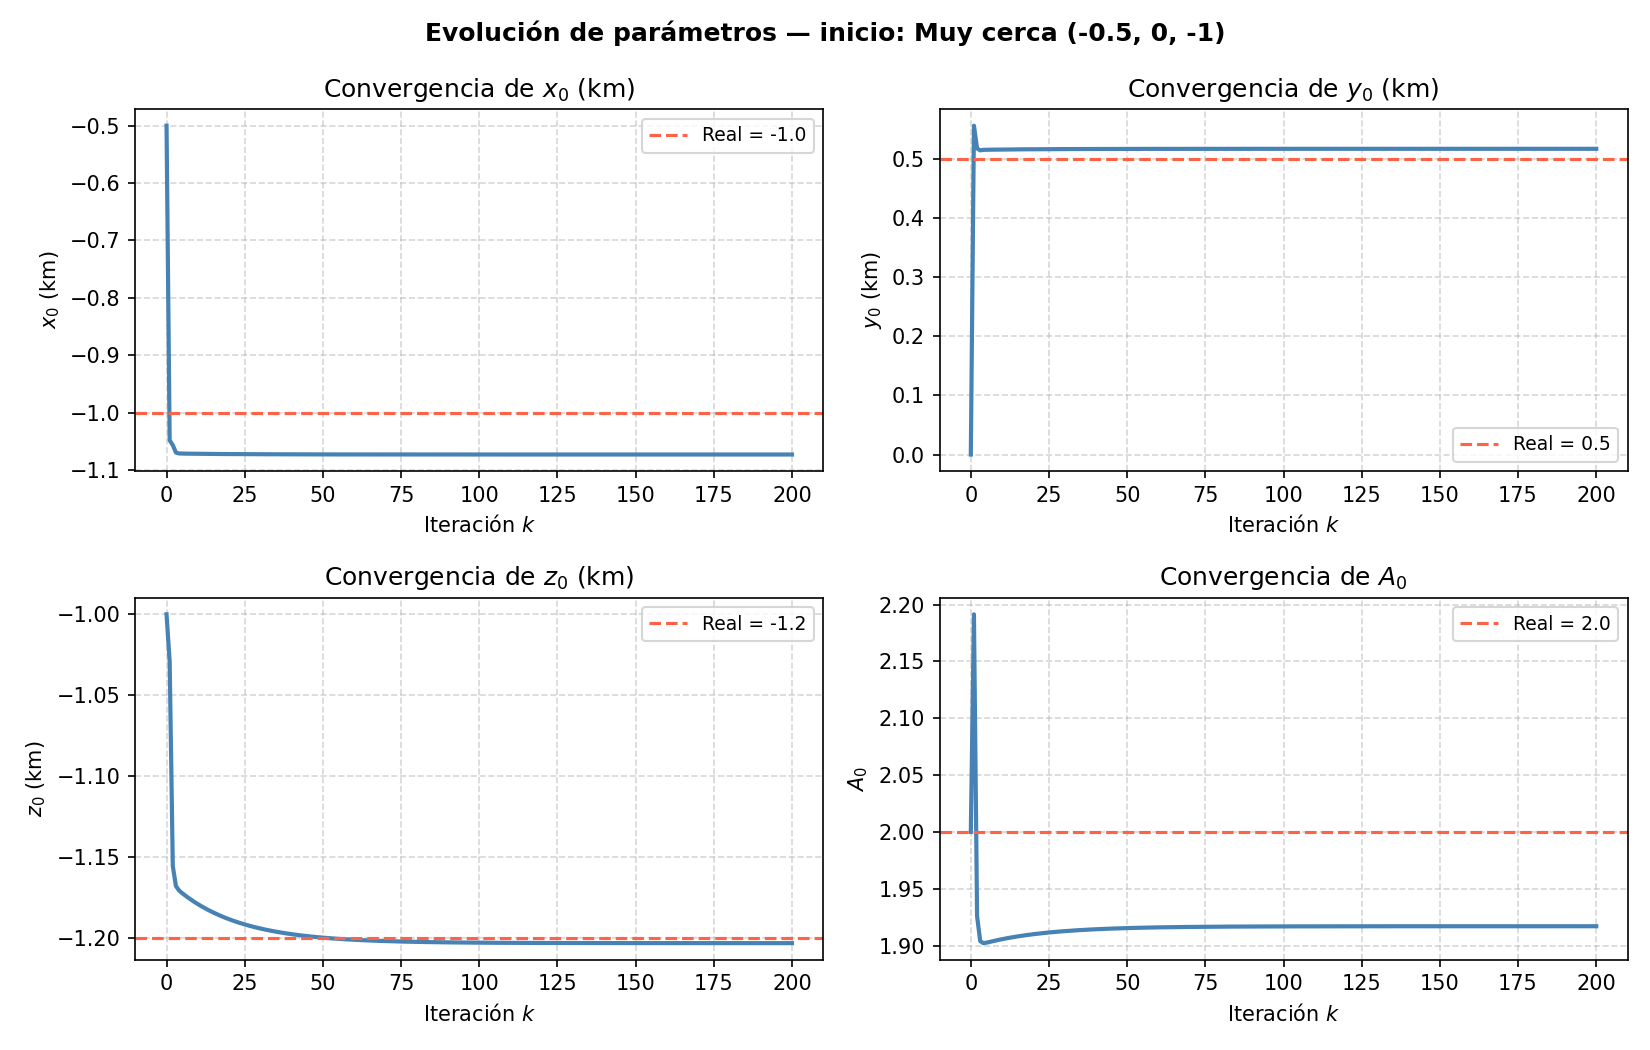
\includegraphics[width=0.90\textwidth]{evolucion_parametros.png}
    \caption{Evolución de cada parámetro $(x_0, y_0, z_0, A_0)$ a
    lo largo de las iteraciones (inicio cercano). Las líneas rojas
    punteadas indican los valores reales. La convergencia de $x_0$
    e $y_0$ es muy rápida; la de $z_0$ y $A_0$ requiere más
    iteraciones, anticipando la mayor incertidumbre intrínseca de
    estos parámetros.}
    \label{fig:param_evol}
\end{figure}

La Tabla~\ref{tab:resultados} resume los resultados de todos los métodos.

\begin{table}[H]
    \centering
    \caption{Comparación de resultados de estimación. Error posicional
    $= \|\hat{\mathbf{r}} - \mathbf{r}_0\|_2$ en km.}
    \label{tab:resultados}
    \begin{tabular}{lrrrrc}
        \toprule
        \textbf{Método / Inicio} &
        $x^*$ & $y^*$ & $z^*$ & $A_0^*$ & \textbf{Err. (km)} \\
        \midrule
        Fuente real                       & $-1.000$ & $0.500$ & $-1.200$ & $2.000$ & --- \\
        \midrule
        F. bruta ($A_0=2$ fijo)           & $-1.051$ & $0.566$ & $-1.212$ & $2.000$ & $0.084$ \\
        F. bruta perfilada                & $-1.051$ & $0.566$ & $-1.151$ & $1.962$ & $0.096$ \\
        \midrule
        L--M — Cerca                      & $-1.073$ & $0.518$ & $-1.203$ & $1.917$ & $0.075$ \\
        L--M — Lejos NE                   & $-1.073$ & $0.518$ & $-1.203$ & $1.917$ & $0.075$ \\
        L--M — Lejos SO                   & $-1.073$ & $0.518$ & $-1.203$ & $1.917$ & $0.075$ \\
        L--M — Muy cerca                  & $-1.073$ & $0.518$ & $-1.203$ & $1.917$ & $0.075$ \\
        \bottomrule
    \end{tabular}
\end{table}

\subsection{Análisis del Hessiano e incertidumbre de los parámetros}
\label{sec:analisis_hessiano}

Aplicando el análisis de la Sección~\ref{sec:teoria_covarianza}
sobre la solución de Levenberg--Marquardt, se obtienen los siguientes
resultados.

\paragraph{Estadística del residual.}
Con $M=8$ y $p=4$, los grados de libertad son $\nu = M - p = 4$. El
residual cuadrático en el mínimo es $E^* = 2.32\times 10^{-8}$, y la
desviación estándar estimada del ruido en los datos es
$\hat{\sigma} = \sqrt{E^*/\nu} = 7.62\times 10^{-5}$. Este valor es
coherente con la magnitud de los $\sigma_i$ generados (Tabla~\ref{tab:datos}).

\paragraph{Barras de error.}
La Tabla~\ref{tab:errores} resume las desviaciones estándar
$\sigma_{m_j}$ obtenidas de $\sqrt{\mathrm{diag}(\widehat{\mathbf{C}})}$,
junto con las incertidumbres relativas.

\begin{table}[H]
    \centering
    \caption{Estimación y barras de error ($1\sigma$) de cada parámetro.}
    \label{tab:errores}
    \begin{tabular}{lrrrr}
        \toprule
        \textbf{Parámetro} & \textbf{Real} & \textbf{Estimado} &
        $\sigma_{m_j}$ & $\sigma_{\text{rel}}$ \\
        \midrule
        $x_0$ (km) & $-1.000$ & $-1.073$ & $0.0345$ & $3.22\%$ \\
        $y_0$ (km) & $ 0.500$ & $ 0.518$ & $0.0354$ & $6.84\%$ \\
        $z_0$ (km) & $-1.200$ & $-1.203$ & $0.5982$ & $49.71\%$ \\
        $A_0$       & $ 2.000$ & $ 1.917$ & $0.2855$ & $14.89\%$ \\
        \bottomrule
    \end{tabular}
\end{table}

La incertidumbre en profundidad ($\sigma_{z_0} = 0.60$~km) es
\emph{aproximadamente $17$ veces mayor} que la incertidumbre horizontal
($\sigma_{x_0}, \sigma_{y_0} \approx 0.035$~km). Esto cuantifica
formalmente la anisotropía de la resolución del problema.

\paragraph{Descomposición espectral.}
Los autovalores de $\mathbf{G}^T\mathbf{G}$ son:
\begin{equation*}
    \lambda_1 = 1.79\times 10^{-3},\quad
    \lambda_2 = 2.64\times 10^{-5},\quad
    \lambda_3 = 8.60\times 10^{-6},\quad
    \lambda_4 = 1.32\times 10^{-8}
\end{equation*}

con número de condición $\kappa = \lambda_1/\lambda_4 = 1.36\times 10^{5}$.
Este valor es indicativo de un problema \emph{mal condicionado}
\cite{golub2013matrix}, lo que explica por qué Gauss--Newton puro
(sin regularización) diverge y justifica el uso de Levenberg--Marquardt
con backtracking.

\begin{figure}[H]
    \centering
    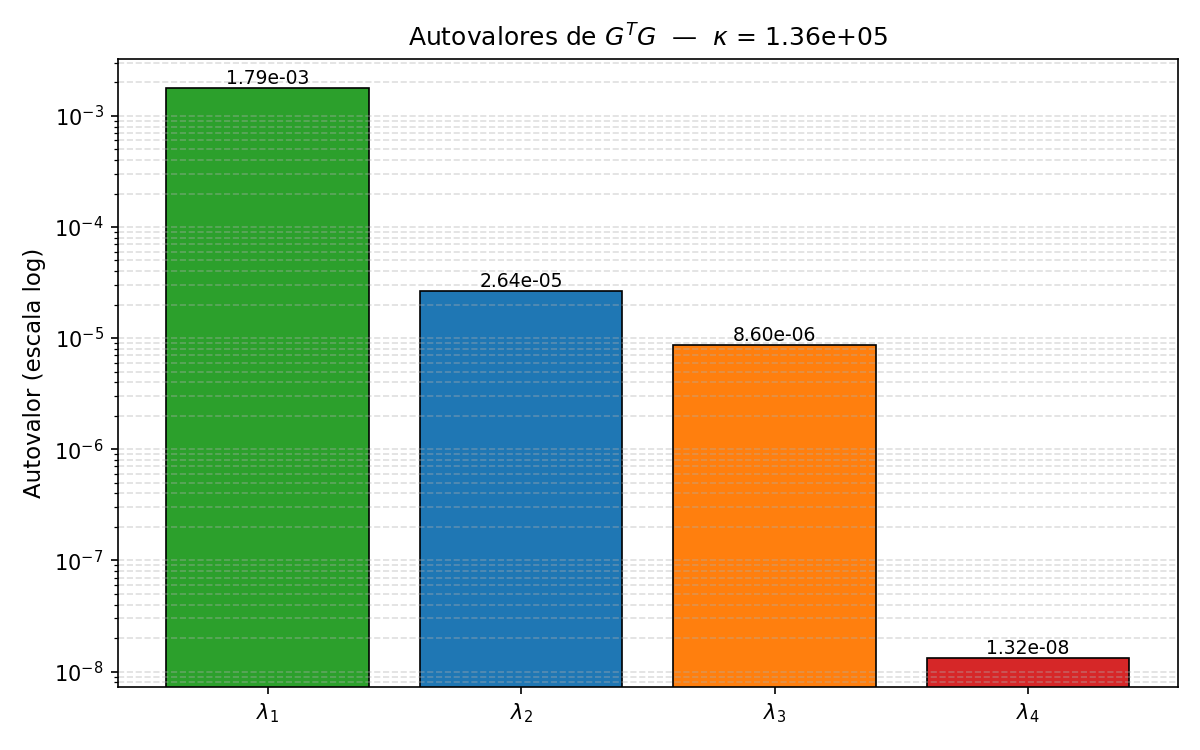
\includegraphics[width=0.85\textwidth]{autovalores_GtG.png}
    \caption{Autovalores de $\mathbf{G}^T\mathbf{G}$ en escala
    logarítmica. La diferencia de cinco órdenes de magnitud entre
    $\lambda_1$ y $\lambda_4$ refleja el mal condicionamiento del
    problema.}
    \label{fig:autovalores}
\end{figure}

\paragraph{Direcciones bien y mal resueltas.}
La Tabla~\ref{tab:autovectores} muestra los autovectores
correspondientes, expresados en la base $(x_0, y_0, z_0, A_0)$:

\begin{table}[H]
    \centering
    \caption{Autovectores de $\mathbf{G}^T\mathbf{G}$. Cada columna
    es una dirección del espacio de parámetros, ordenadas de mejor
    ($\mathbf{v}_1$, mayor autovalor) a peor resuelta ($\mathbf{v}_4$,
    menor autovalor).}
    \label{tab:autovectores}
    \begin{tabular}{lrrrr}
        \toprule
        & $\mathbf{v}_1$ (mejor)
        & $\mathbf{v}_2$
        & $\mathbf{v}_3$
        & $\mathbf{v}_4$ (peor) \\
        \midrule
        $x_0$ & $-0.892$ & $+0.015$ & $-0.449$ & $-0.049$ \\
        $y_0$ & $-0.160$ & $+0.924$ & $+0.344$ & $+0.047$ \\
        $z_0$ & $+0.213$ & $+0.202$ & $-0.320$ & $\mathbf{-0.901}$ \\
        $A_0$ & $+0.364$ & $+0.324$ & $-0.761$ & $\mathbf{+0.429}$ \\
        \bottomrule
    \end{tabular}
\end{table}

\begin{figure}[H]
    \centering
    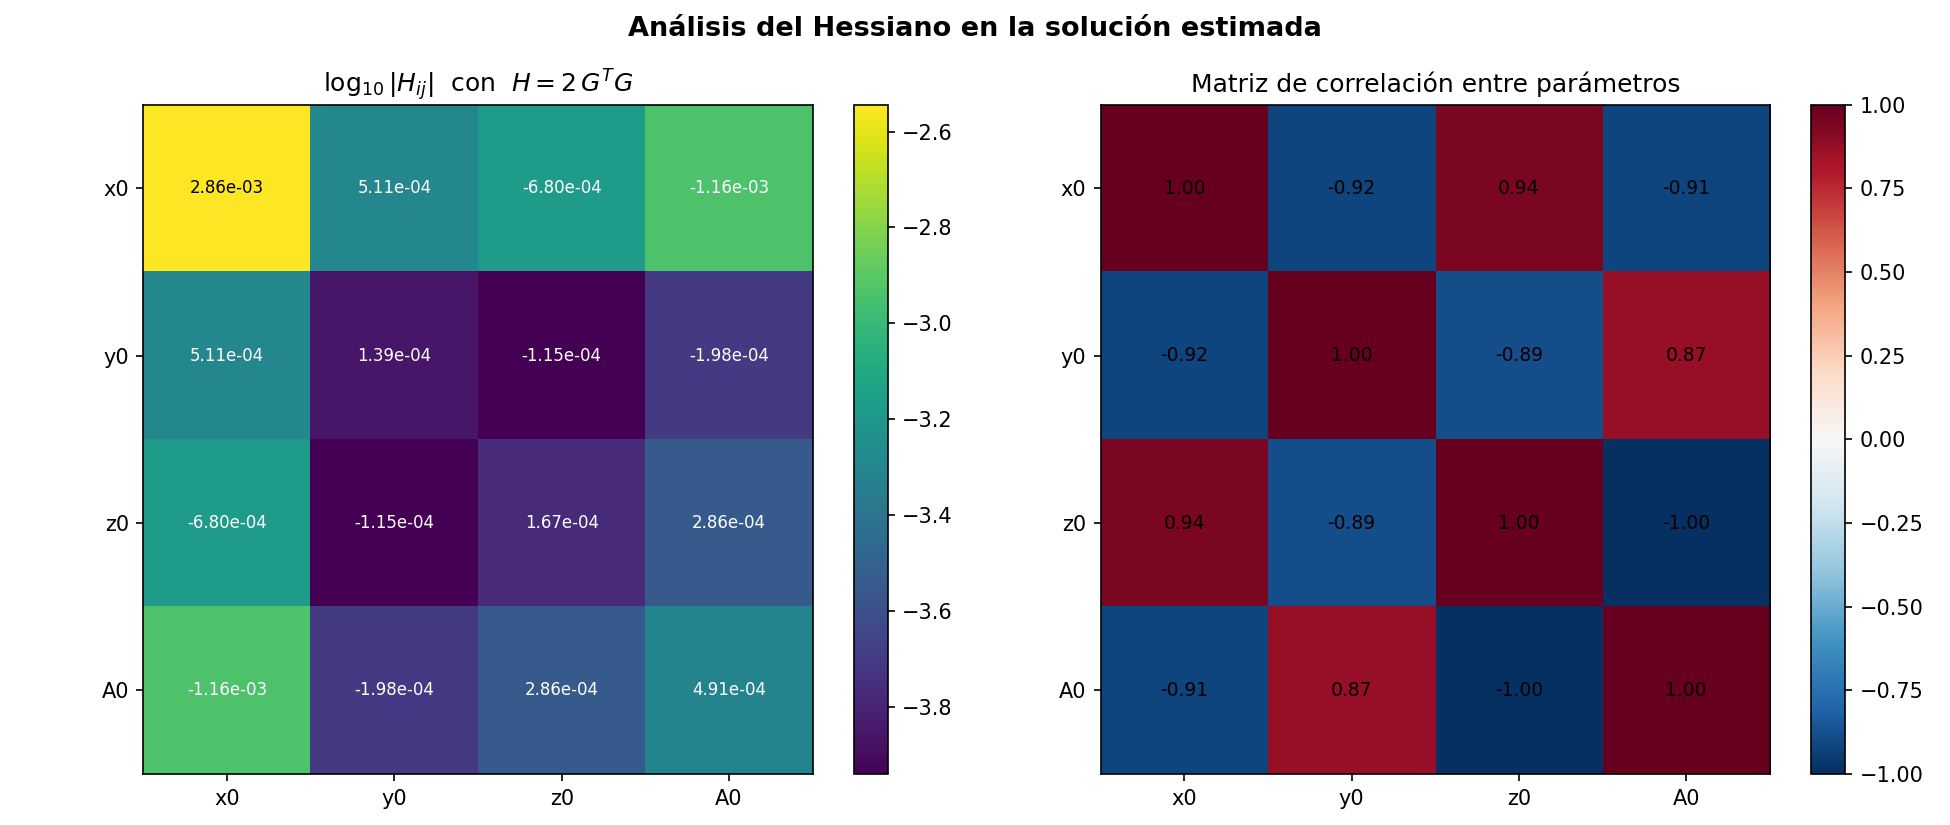
\includegraphics[width=0.97\textwidth]{hessiano_correlacion.png}
    \caption{Izquierda: Hessiano $H = 2\mathbf{G}^T\mathbf{G}$ en
    escala logarítmica. Derecha: matriz de correlación entre los
    cuatro parámetros estimados. La correlación negativa fuerte
    entre $z_0$ y $A_0$ es la firma del trade-off
    profundidad--amplitud.}
    \label{fig:hessiano_corr}
\end{figure}

\begin{figure}[H]
    \centering
    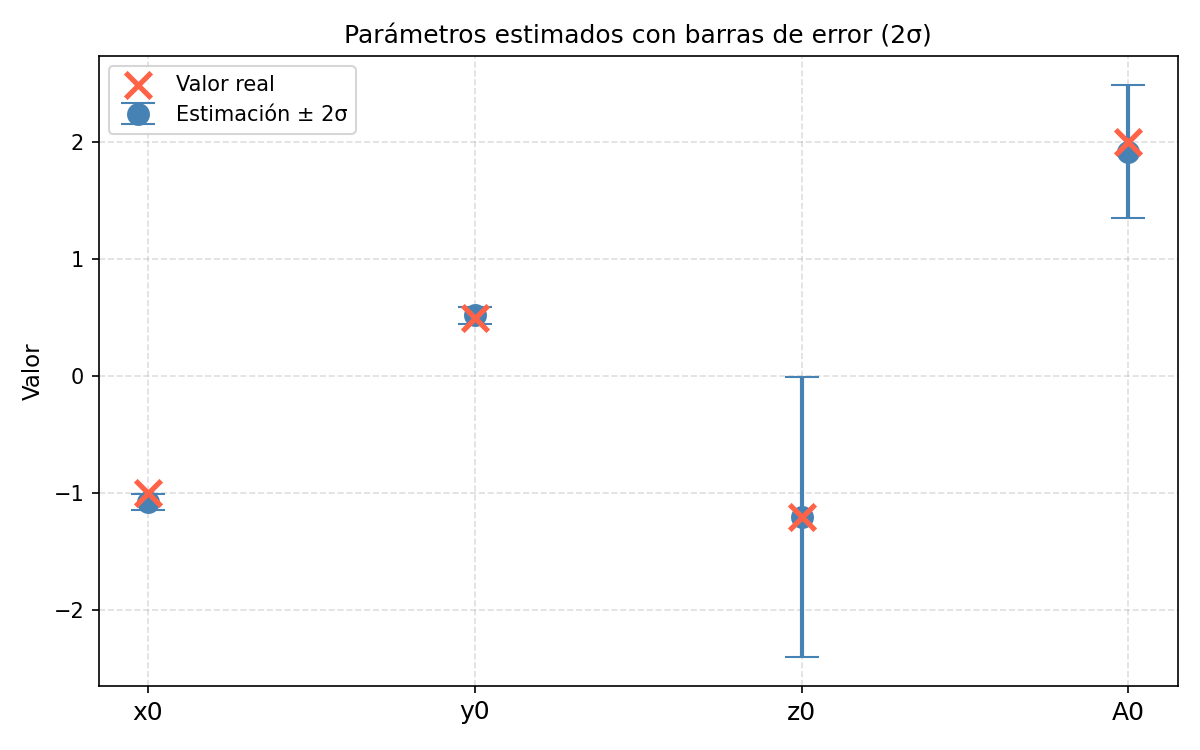
\includegraphics[width=0.85\textwidth]{parametros_con_error.png}
    \caption{Parámetros estimados (puntos azules) con barras de error
    de $\pm 2\sigma$, comparados con los valores reales (cruces rojas).
    Las grandes barras en $z_0$ y $A_0$ son la manifestación
    cuantitativa del mal condicionamiento del problema.}
    \label{fig:param_errores}
\end{figure}

%----------------------------------------------------------
% 6. ANÁLISIS Y DISCUSIÓN
%----------------------------------------------------------
\section{Análisis y Discusión}

\subsection{Forma y estructura de la función de error}

La función $E(x,y,z)$ es una suma de ocho términos cuadráticos, cada
uno asociado a una estación. En los mapas de calor
(Figura~\ref{fig:heatmaps}) se aprecia una estructura de
\textit{embudo}: valores altos en la periferia del dominio y una zona
oscura concentrada alrededor del mínimo. En el corte óptimo
(Figura~\ref{fig:heatmap_opt}), los contornos elipsoidales indican
curvatura similar en $x$ e $y$, es decir, igual sensibilidad a
desplazamientos en ambas direcciones horizontales.

\subsection{Unicidad del mínimo}

La unicidad del mínimo se establece de manera \emph{empírica}: los
cuatro puntos de partida del método iterativo —incluyendo uno a más
de $7$~km de la solución— convergen exactamente al mismo punto final
$(x^*, y^*, z^*, A_0^*) = (-1.073, 0.518, -1.203, 1.917)$. Si
existieran mínimos locales secundarios, distintos inicios convergerían
a distintas soluciones. Adicionalmente, el análisis del Hessiano
muestra que $\mathbf{G}^T\mathbf{G}$ es definido positivo
($\lambda_4 = 1.32\times 10^{-8} > 0$), lo que confirma localmente que
el punto crítico encontrado es un mínimo y no un punto de silla.

Las únicas regiones de valor casi constante son las esquinas del
dominio, donde todos los residuales son grandes pero similares entre
sí. Estas constituyen mesetas de error alto, no mínimos locales, y no
interfieren con la estimación.

\subsection{Sensibilidad respecto a z}
\label{sec:sensibilidad_z}

El hallazgo más importante del análisis es que \textbf{la función de
error es significativamente menos sensible a la profundidad} que a las
coordenadas horizontales. Esto se manifiesta en tres mediciones
\emph{independientes} y \emph{coincidentes}:

\begin{enumerate}[leftmargin=*, itemsep=2pt]
    \item El \textbf{ancho local del pozo} de $E_{\min}(z)$ es de
    $0.132$~km, pero el rango de valores de $z$ donde
    $E_{\min}(z) \lesssim 10 E^*$ alcanza casi $1$~km.
    \item La \textbf{incertidumbre formal} obtenida del Hessiano es
    $\sigma_{z_0} = 0.60$~km, frente a $\sigma_{x_0} \approx
    \sigma_{y_0} \approx 0.035$~km. La razón es de aproximadamente
    $17:1$.
    \item El \textbf{peor autovector} de $\mathbf{G}^T\mathbf{G}$
    está dominado por la componente $z_0$ con magnitud $0.901$ (el
    $90\%$ de la dirección).
\end{enumerate}

Esta anisotropía tiene dos causas físicas:

\begin{enumerate}[leftmargin=*]
    \item \textbf{Geometría superficial de la red.} Todas las
    estaciones están en $z_i \in [-0.5, 0]$~km. Un desplazamiento
    horizontal de la fuente es detectable porque cambia la distancia
    relativa a estaciones distribuidas azimutalmente. Un desplazamiento
    vertical, en cambio, afecta a todas las estaciones de forma similar
    porque éstas están casi coplanarias, produciendo un cambio
    \emph{global} en las amplitudes que se confunde con un cambio en
    $A_0$.

    \item \textbf{Acoplamiento $z_0$--$A_0$.} El cuarto autovector
    confirma directamente este acoplamiento: las componentes de $z_0$
    ($-0.90$) y $A_0$ ($+0.43$) tienen signos opuestos. La interpretación
    es que existe una dirección del espacio de parámetros a lo largo de
    la cual las amplitudes predichas casi no cambian: aumentar $|z_0|$
    (fuente más profunda) compensado con un aumento proporcional de
    $A_0$ produce amplitudes virtualmente indistinguibles para una
    red superficial.
\end{enumerate}

Este fenómeno, conocido como \emph{depth--amplitude trade-off}, es
bien documentado en sismología \cite{thurber1985nonlinear,
husen2010earthquake} y motiva el uso de redes con estaciones de
distintas profundidades en escenarios reales.

\subsection{Comparación de los tres métodos}

La Tabla~\ref{tab:resultados} permite contrastar los tres enfoques:

\paragraph{Fuerza bruta con $A_0 = 2$ fijo (error: $0.084$~km).}
Esta versión utiliza información \emph{a priori perfecta} sobre
$A_0$. La limitación es la resolución de la grilla:
$\Delta x = \Delta y = 0.16$~km implica un error en $x$ e $y$ del orden
de $\Delta x/2$, coherente con los $0.05$--$0.07$~km observados.

\paragraph{Fuerza bruta perfilada (error: $0.096$~km).}
Esta versión \emph{estima los cuatro parámetros simultáneamente}
mediante la fórmula analítica de $\widehat{A}_0$
(Ec.~\ref{eq:A0_perfilado}). El error posicional es ligeramente mayor
que en la versión anterior porque al no fijar $A_0$, el método
debe distribuir la información del ruido entre los cuatro parámetros,
y el trade-off $z_0$--$A_0$ desplaza $z^*$ hacia un valor ligeramente
más superficial ($-1.151$~km). La estimación $\widehat{A}_0 = 1.962$
es muy próxima al valor real $2.0$, validando la fórmula.

\paragraph{Levenberg--Marquardt (error: $0.075$~km).}
El método iterativo no está limitado por la resolución discreta y
alcanza el menor error posicional. Los cuatro inicios convergen al
\emph{mismo} punto, confirmando empíricamente la unicidad del mínimo.
La convergencia es robusta gracias al backtracking adaptativo:
inicios cercanos requieren aproximadamente $30$ iteraciones; inicios
lejanos hasta $110$.

\paragraph{Consistencia entre métodos.}
Es importante notar que ambos métodos que estiman $A_0$ libremente
(perfilada e iterativo) obtienen valores $\widehat{A}_0$ similares
($1.96$ y $1.92$ respectivamente), \emph{ambos por debajo} del valor
real $2.0$. Esta coincidencia no es casualidad: es el efecto del
ruido específico de la realización con \texttt{seed} $=42$,
materializado en la dirección del autovector $\mathbf{v}_4$.

\subsection{Validez de las barras de error}

Las barras de error de $\pm 2\sigma$ (intervalo de confianza nominal
del $95\%$) cubren los valores reales en tres de los cuatro parámetros
($y_0$, $z_0$ y $A_0$). El valor real $x_0 = -1.000$ queda apenas
\emph{fuera} del intervalo $[-1.142, -1.004]$, una diferencia de solo
$4\times 10^{-3}$~km. Esto sugiere un ligero sesgo en $x_0$ debido al
ruido específico de esta realización, pero está dentro del margen
estadísticamente esperable cuando se evalúa a $95\%$ con un solo
experimento. Una evaluación verdadera de la cobertura requeriría
realizar simulaciones \emph{Monte Carlo} con múltiples realizaciones
del ruido, lo que constituye una extensión natural de este trabajo
(Sección~\ref{sec:trabajo_futuro}).

\subsection{Interpretación física de los resultados}

\textbf{Calidad de la red.} La distribución azimutal completa de las
ocho estaciones es suficiente para determinar unívocamente la posición
horizontal de la fuente. Los autovectores $\mathbf{v}_1$ y $\mathbf{v}_2$,
dominados por $x_0$ y $y_0$ respectivamente, son evidencia directa
de que el sistema $\mathbf{G}\Delta\mathbf{m} = \Delta\mathbf{A}_z$
está bien restringido en estas direcciones.

\textbf{Efecto del ruido.} Con $\alpha = 0.05$, el error posicional
de $0.075$~km representa el \textit{piso de ruido} del método: es la
incertidumbre irreducible dada por la magnitud del ruido y la
geometría del sistema. Reducir $\alpha$ reduciría proporcionalmente
las barras de error.

\textbf{Importancia del trade-off $z_0$--$A_0$.} Si en un escenario
real se conociera $A_0$ con precisión (por ejemplo, por calibración
del instrumento o por información de eventos similares), la
incertidumbre en $z_0$ se reduciría drásticamente. Esta es la
justificación principal del uso de redes calibradas y bases de datos
históricas en sismología operacional \cite{waldhauser2000double}.

%----------------------------------------------------------
% 7. CONCLUSIONES
%----------------------------------------------------------
\section{Conclusiones}

\begin{enumerate}

    \item \textbf{Función de error.} Se construyó exitosamente
    $E(x,y,z)$ como suma de cuadrados de residuales y, adicionalmente,
    se introdujo la versión perfilada $\widetilde{E}(x,y,z)$ que
    incorpora la estimación analítica de $\widehat{A}_0$. Ambas
    funciones presentan un único mínimo global bien definido con
    estructura de embudo y contornos elipsoidales coherentes con la
    geometría del arreglo.

    \item \textbf{Mapas de calor.} La exploración de cortes $z = k$
    permitió visualizar cómo el mínimo horizontal se concentra
    progresivamente conforme $z$ se aproxima a la profundidad real,
    confirmando visualmente la coherencia entre la formulación y la
    realización numérica.

    \item \textbf{Curva $E_{\min}(z)$.} La función reducida presenta un
    mínimo en $z^* = -1.212$~km, con error de $0.012$~km respecto al
    valor real. El \textbf{ancho local del pozo}, calculado mediante
    ajuste parabólico de la segunda derivada (cálculo multivariable
    aplicado directamente), es de $0.132$~km, reflejo de la resolución
    del problema en profundidad.

    \item \textbf{Tres métodos consistentes.} Los tres enfoques de
    estimación (fuerza bruta con $A_0$ fijo, fuerza bruta perfilada y
    Levenberg--Marquardt) producen soluciones consistentes con errores
    posicionales menores a $0.1$~km. El método iterativo alcanza el
    menor error ($0.075$~km), mientras que la fuerza bruta perfilada
    proporciona la comparación metodológicamente más justa al estimar
    los mismos cuatro parámetros que el iterativo.

    \item \textbf{Análisis del Hessiano.} El cálculo formal de la
    matriz de covarianza $\widehat{\mathbf{C}} = \hat{\sigma}^2
    (\mathbf{G}^T\mathbf{G})^{-1}$ permite cuantificar la incertidumbre
    de los parámetros. Se obtiene $\sigma_{z_0} \approx 0.60$~km,
    aproximadamente $17$ veces la incertidumbre horizontal. El número
    de condición $\kappa = 1.36\times 10^{5}$ confirma que el problema
    está mal condicionado, lo que justifica el uso de regularización.

    \item \textbf{Trade-off profundidad--amplitud.} El autovector
    asociado al menor autovalor de $\mathbf{G}^T\mathbf{G}$ está
    dominado por $z_0$ ($-0.90$) con componente opuesta en $A_0$
    ($+0.43$), constituyendo \emph{evidencia cuantitativa directa}
    del acoplamiento $z_0$--$A_0$ conocido en sismología. Este
    resultado es el aporte más distintivo del análisis y no es
    accesible a simple vista en los mapas de calor.

    \item \textbf{Robustez del método de Levenberg--Marquardt.} El
    esquema con backtracking adaptativo y filtro físico ($A_0 > 0$)
    converge de forma confiable desde inicios muy lejanos del óptimo
    real, superando las limitaciones de Gauss-Newton puro que diverge
    en este problema mal condicionado.

    \item \textbf{Limitaciones del modelo.} El modelo de atenuación
    es una simplificación: no considera heterogeneidad del medio,
    anisotropía, efectos de superficie ni tipos de ondas distintos.
    Estas limitaciones restringen su aplicabilidad a contextos reales,
    pero son apropiadas para el objetivo académico de este proyecto.

\end{enumerate}

\subsection*{Trabajo futuro}
\label{sec:trabajo_futuro}

Las extensiones naturales del proyecto incluyen:

\begin{itemize}[leftmargin=*, itemsep=2pt]
    \item \textbf{Simulaciones Monte Carlo} con $N \sim 500$ semillas
    aleatorias distintas para evaluar empíricamente la distribución
    de los estimadores y la cobertura real de los intervalos de
    confianza.
    \item \textbf{Inversión bayesiana} mediante muestreo MCMC para
    obtener distribuciones posteriores completas en lugar de
    aproximaciones gaussianas.
    \item \textbf{Estaciones a distintas profundidades} para reducir
    la anisotropía de la resolución en $z$.
    \item \textbf{Modelos de atenuación más realistas} incluyendo
    factores como $Q$ (factor de calidad), velocidades dependientes
    de la profundidad y geometría esférica.
\end{itemize}

%----------------------------------------------------------
% 8. REFERENCIAS
%----------------------------------------------------------
\newpage
\bibliography{referencias}
\bibliographystyle{IEEEtran}

%----------------------------------------------------------
% 9. ANEXOS
%----------------------------------------------------------
\appendix

\section{Repositorio de código}
\label{apx:repo}

El código fuente completo del proyecto, incluyendo todos los scripts
de análisis y los datos generados, está disponible en:

\begin{center}
    \url{https://github.com/Fabiann1809/fuenteSismicaCalculo}
\end{center}

Estructura del repositorio:
\begin{itemize}
    \item \texttt{datos/} — Estaciones, parámetros del sismo y
    resultados precalculados (JSON).
    \item \texttt{src/} — Módulos del modelo físico: \texttt{modelo.py},
    \texttt{ruido.py}, \texttt{funcion\_error.py}, \texttt{jacobiano.py},
    \texttt{utilidades.py}.
    \item \texttt{analisis/} — Scripts numerados por fase:
    \begin{itemize}
        \item \texttt{01\_simular\_datos.py} — Generación de datos
        sintéticos.
        \item \texttt{02\_exploracion\_error.py} — Exploración por
        grilla 3D, mapas de calor.
        \item \texttt{03\_curva\_emin.py} — Curva $E_{\min}(z)$ y
        análisis de curvatura local.
        \item \texttt{04\_metodo\_iterativo.py} —
        Levenberg--Marquardt y comparación.
        \item \texttt{05\_generar\_video.py} — Animación de los
        cortes en $z$.
        \item \texttt{06\_analisis\_hessiano.py} — Covarianza,
        autovalores y barras de error.
        \item \texttt{07\_fuerza\_bruta\_perfilada.py} — Función
        de error perfilada con $\widehat{A}_0$ analítico.
    \end{itemize}
    \item \texttt{figuras/} — Todas las gráficas generadas.
    \item \texttt{video/} — Animación de mapas de calor.
    \item \texttt{docs/} — Documento \LaTeX{}.
\end{itemize}

\section{Figuras adicionales}

\begin{figure}[H]
    \centering
    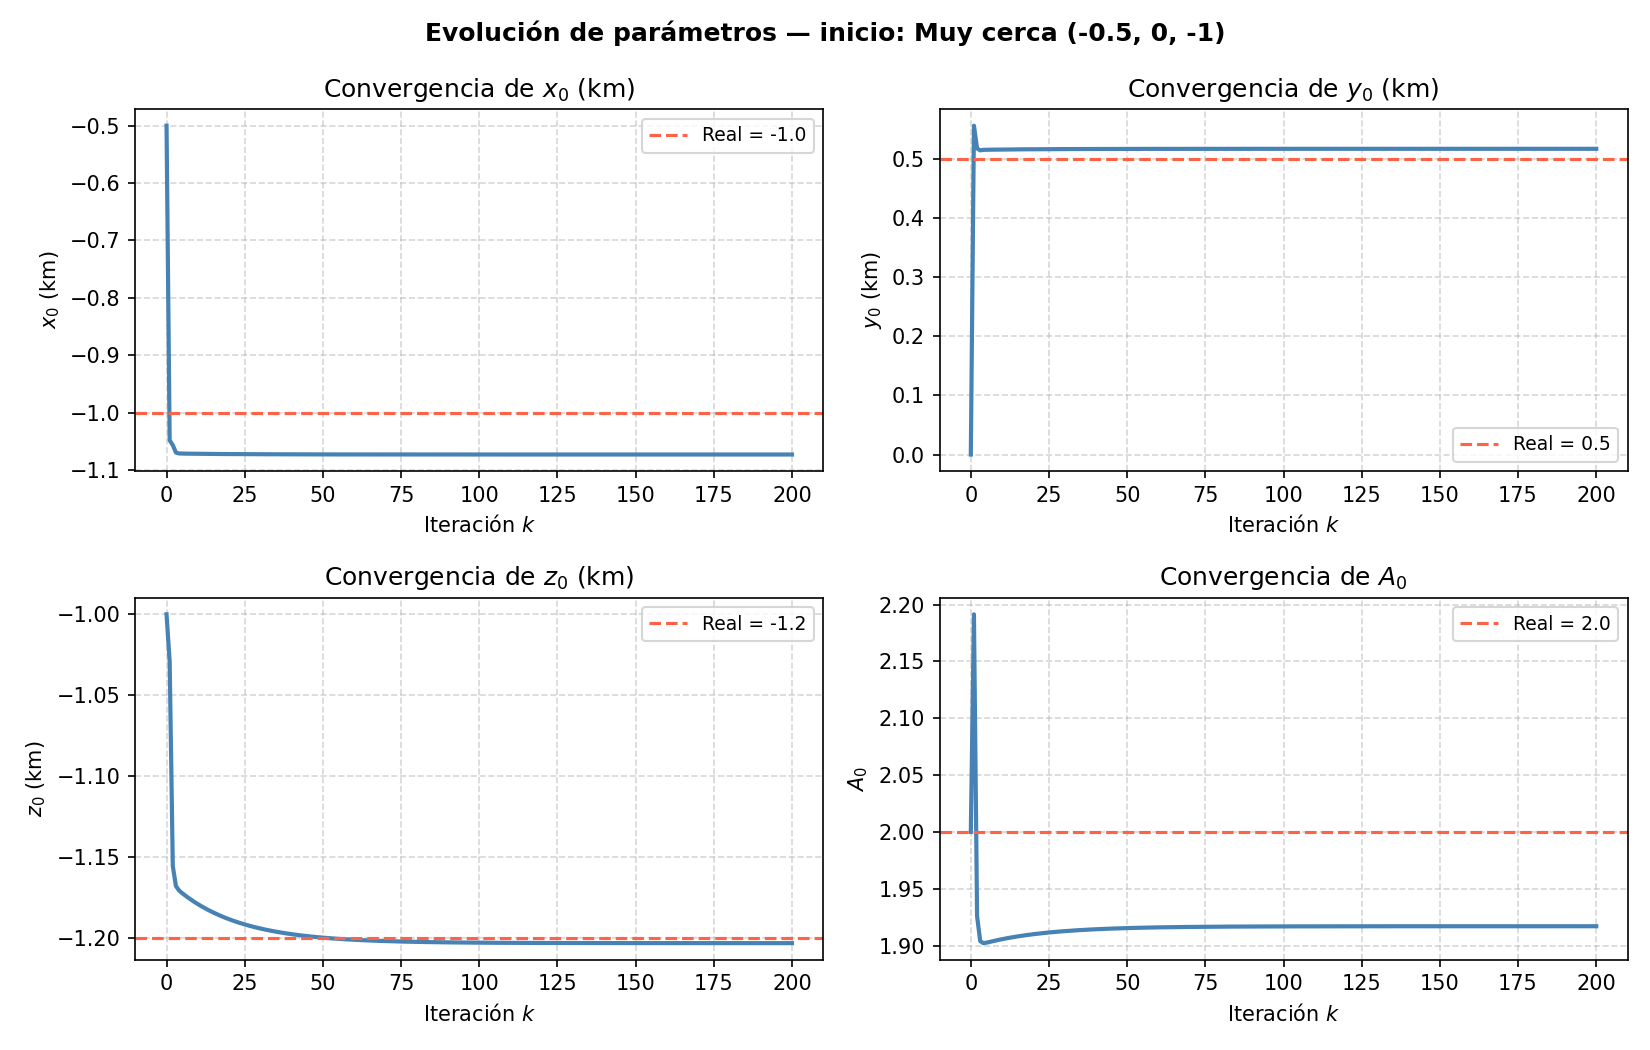
\includegraphics[width=0.90\textwidth]{evolucion_parametros.png}
    \caption{Evolución de los cuatro parámetros del modelo a lo largo
    de las iteraciones (inicio cercano). Se aprecia la convergencia
    rápida en las primeras iteraciones, especialmente para $x_0$ e
    $y_0$, mientras que $z_0$ y $A_0$ requieren más iteraciones para
    estabilizarse, reflejando el trade-off $z_0$--$A_0$ identificado
    en el análisis del Hessiano.}
\end{figure}

\section{Video de animación}

La animación de los $100$ mapas de calor $E(x,y,z=k)$ para
$k\in[-3, 0]$~km, con el cursor de la curva $E_{\min}(z)$ en el panel
lateral, está disponible en:

\begin{center}
    \url{https://github.com/Fabiann1809/fuenteSismicaCalculo/blob/main/video/mapa_calor_sismica.gif}
\end{center}

%==========================================================
\end{document}
%==========================================================